\documentclass[a4paper,12pt]{article}
\usepackage{graphicx}
\usepackage{titling}
\usepackage{color}
\newcommand{\subtitle}[1]{%
  \posttitle{%
    \par\end{center}
    \begin{center}\large#1\end{center}
    \vskip0.5em}%
}
\usepackage{color}
\usepackage{tabularx}
\usepackage{array,multirow}
\definecolor{light-gray}{gray}{0.80}
\usepackage{url}
\usepackage{listings}
\usepackage[tight,footnotesize]{subfigure}  
\usepackage[top=2cm, bottom=2cm, left=4cm, right=2cm]{geometry}
\usepackage{amsmath}
\usepackage{float}
%\begin{titlepage}
%\begin{center}
\title{Processing Geospatial Data in BaseX}
\subtitle{Master Thesis in fulfillment of the requirements for the degree of
Master of Science (M.Sc.)}
%\subtitle{Submitted to the Department of Computer and Information Science at the
%University of Konstanz
%}
%{ \huge \bfseries Processing GeoSpatial Data in BaseX \\[0.4cm] }
%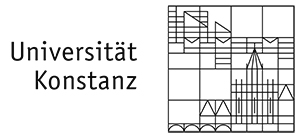
\includegraphics[width=0.15\textwidth]{./unisignet-klein}~\\[1cm]
\author{\\\\Author: \\
	Masoumeh Seydi
	\\\\\\Supervisors: \\
	Prof. Dr. Marc H. Scholl \\ 
	\\\\\\
	Konstanz University}
%\end{center}
%\end{titlepage}
\begin{document}
\definecolor{darkgray}{gray}{0.35}
\lstnewenvironment{fakeXML}[1][]{
\lstset{basicstyle=\footnotesize\sffamily,
linewidth=\linewidth,
breaklines=true, 
%numbers=left,
%stepnumber=1,
%numbersep=10pt,
frame=single,
framerule=1.0pt,
%backgroundcolor=\color{darkgray},
language=HTML,
%identifierstyle=\color[rgb]{1,0,0},
%emph={intersects}, emphstyle=\color{red},
%keywordstyle=\color[rgb]{0,0,1},
%commentstyle=\color[rgb]{0.133,0.545,0.133},
%stringstyle=\color[rgb]{0.627,0.126,0.941},
morekeywords={xml, ref, xs, version, targetNamespace, minOccurs, maxOccurs}
}\lstset{#1}}{}

\lstnewenvironment{fakeJSON}[1][]{
\lstset{
basicstyle=\footnotesize\sffamily,
linewidth=\linewidth,
breaklines=true,
%escapeinside={\%*}{*)}
%numbers=left,
%stepnumber=1,
%numbersep=10pt,
%frame=single,
%framerule=1.0pt,
language=HTML,
emph={}
}\lstset{#1}}{}


\renewcommand{\lstlistingname}{Code}


\maketitle
\thispagestyle{empty}

\newpage
\section*{Abstract}
Geospatial information has been growing exponentially and has been used in variety of applications such as GIS, bioinformatics, and decision support systems. 
Variety of applications have demanded efficient approaches of data manipulation to cover their requirements. 
The XML-based data representation and manipulation in this field is one of these approaches that also has been considered and applied by databases, especially native XML databases. 
%The open-source software BaseX is one of these native XML databases. 

This work tries to investigate the challenges of geospatial data processing in BaseX~\cite{www/basex}, an open-source native XML database, by discussing the issues in geospatial querying, geospatial functionalities, and query efficiency. 
At first, this thesis starts with introducing a number of indexing approaches as various ways of efficient geospatial data manipulation. 
Next, general geospatial functionalities in some similar databases are investigated. 
Then, the geospatial features for GML~\cite{gml} data representation are added to BaseX, 
using the JTS library~\cite{jts} and based on the EXPath specification.
%The geospatial query is adpated also in the structure of BaseX. 

To improve the performance of spatial queries, an indexing structure is applied as an external library.
%the data is indexed by the indexing structure STR-tree.
At the end, we have tried another querying approach by connecting to MongoDB, a powerful document-based database system, through BaseX as an effort to find other efficient ways.
Evaluations in various stages and provided advantages and disadvantages of different approaches can be considered in deciding on future developments in BaseX.
\thispagestyle{empty}

\newpage
\section*{Acknowledgments}
\thispagestyle{empty}

The completion of this master thesis would not have been possible 
without the support of many people. 
I must express my sincerest thanks towards 
Dr. Christian Gr{\"u}n for his continuous support and patience during my research.
I should confess that I can not imagine a better person to guide and advise me. Besides, I would like to extend my gratitude to my supervisor Prof. Dr. Marc H. Scholl to give me the chance to be involved in this group.

My special appreciation also goes to Dr. Rolf A. de By from the University of Twente for
answering completely and accurately the questions that I would ask
frequently and providing me a sample data set to test. I would like to offer my heartfull gratitude my parents and family for encouraging me 
throughout my whole study. At the end, I am deeply appreciative of my beloved, M. Ali Rostami, without whom it would have been impossible to continue.


\newpage
\tableofcontents

\thispagestyle{empty}
\newpage
\section{Introduction}
\setcounter{page}{1}
Geospatial data supports a wide range of ever-expanding applications in various scientific, governmental, business, and industrial areas such as geoscience, energy exploration, natural resource management, disaster management, transportation engineering, and urban planning. 
Numerous researches and efforts have been dedicated to make the most efficient use of this data, either in representation or manipulation. 
XML-based structures are parts of the widely used standards to represent the complex structure of geospatial data. 
Geographic Information Systems (GIS)~\cite{gis-intro}, traditional databases, and other systems have been developed or adopted to handle this type of data format. 
Storage and retrieval of XML-based geospatial data in native XML databases are also suitable ways to fulfill the geospatial requirements. This requires adding geospatial functionalitie as a starting point.

Our contribution is to add geospatial functionalities to BaseX with the support of \emph{Geography Markup Language (GML)} as a geospatial data format. 
To do the spatial operations on GML, existing open source libraries are applied.
The big challenge of implementation is the effectiveness of operations
since geospatial data is often huge in size and complex in structure.
Hence, performance improvement of data retrieval from such a data structure 
needs special efforts. 

Spatial indexing structures are common solutions to improve query performance according to specific constraints and properties of spatial data.
As various spatial index algorithms consider different requirements, choosing a proper index should be based on our individual system properties.
We have followed this purpose first throught a short study over a huge set of indexing structures.
% and then an overview of the geospatial features in similar database systems.
%the following tasks,
%\begin{itemize}
%\item a short study over a huge set of indexing structures
%\item an overview of the geospatial features in similar database systems,
%\end{itemize}
%to find the most proper approach in providing geospatial functionalities in BaseX. 
Since the number of indexing structures are large, 
we have selected the structures among the most widely accepted ones in the literature.
The goal of this study is to add a new source of discussion 
for these structures that helps to understand them more effectively for further developments in BaseX. 
However there are other efforts discussing the index structures, 
here we provide a comprehensible explanation and different prespectives which are collected from various sources.
To make a quick and efficient overview over these structures, 
we add a short summary explaining the indexing structures, advantages, and disadvantages.
This summary helps to decide the optimum structure for our approach. 

Then, an overview of the geospatial features in similar database systems is provided. Since the database systems with geospatial functionalities are practical samples, this overview can help us to gain an insight into the different ways of implementation% of geospatial functionalities,
%some other database systems with the geospatial ability are practical samples.
In this part we expalin how the geospatial functionlities are provided in each database.
Furthermore, the indexing structures together with different abilities
supplied by each of these databases are discussed briefly.

In the next steps, we develop the \textit{Geo Module} together with an indexing structure in BaseX.
Evaluation of this module using the real-world data
comes hereafter to demonstrate the efficiecny of implementation.
As an experimental way towards more effective geospatial features, 
we provide a driver to connect to the well-known document-based database MongoDB.
Throught this connection, the queries which are written in BaseX, are executed in MongoDB and then the results are accessible via BaseX. This approach can benefit from the spatial index structure and other spatial functionalities of MongoDB. 
We compare the query time and indexing via this connection with the direct query on BaseX. 
These results and evaluations are the basis for further investigations and developments in BaseX. 
%time complexity is especially of great interest. 
%We talk about the motivations to ....
%chera XML khube.......

%\subsection{Motivation}
%BaseX~\cite{www/basex} is a high-performance XML~\cite{www/xml}
% database which is developed in Konstanz university.
%It has a powerful text processor as well as the full support 
%for XQuery~\cite{www/xquery,www/xqueryfun} language according to \cite{conf/xsym/GrunGHS09}.
%Our goal is to empower BaseX to process the geospatial data in an efficient way. This means to add the support of handling \emph{Geography Markup Language (GML)} data. 
%The Open Geospatial Consortium (OGC)
%which is an internationally recognized organization for geospatial standards,
%is defined this new special XML grammar for the geographical data.
%We want to have a complete support of this language in BaseX
%which means the abilities to read, write, and query this data.
%To achieve this goal we need extensive knowledge over existing researches on the geospatial data and specifically indexing techniques. In this work, a short survay is .....
%we also consider the othe xml databases to find the best solutions....

%\subsection{Overview}
This thesis is structured as follows. We first start with the definitions of concepts needed later in the discussions
in Section~\ref{s.method}. In addition, a number of spatial indexing structures are introduced in this section. 
%the basic geospatial data and it's application areas will be introduced. 
Then, Section~\ref{s.rwork} explains related works in various areas in geospatial processing. The implementation of the Geo Module in BaseX is described in Section~\ref{s.basex}. 
Towards more efficient ways, an approach is experienced by connecting to MongoDB which is evaluated in Section~\ref{s.mongo}.
% the efficiency of the module
%by proposing another way considering MongoDB.
At the end, ideas for further works are summarized in
Section~\ref{s.future}.


\newpage
\section{Geospatial Data Processing}
\label{s.method}
%TODO:in tarifa bere bakhshe badi, inja chanta jomle koli begam
According to \emph{Collins} dictionary, the word \emph{geospatial} is an adjective relating to a position of things on Earth's surface, also \emph{geospatial data} is the data representing any thing on Earth's surface. Regarding the importance of geospatial data, many standards and systems have been developed  during the years to manipulate, represent and make use of them. Countries and organizations are using different systems and standards to represent geospatial data and consequently there are numerous systems to fulfill a range of requirements. A an example, the World Geodesic System (WGS) is one of these systems that is commonly used all around the world. WGS84 is the latest version of this standard which
was introduced in $1984$ and is widely used for expressing the locations on Earth in wide range of services, including satellite services, notably Global Positioning System (GPS), and Google Maps which employ this system as a reference.

In this section, we mainly explain some existing geospatial indexing structures as the most critical part of geospatial data processing in database systems. After some basic definitions in Section \ref{termsanddef}, geospatial data processing in XML~\cite{www/xml} databases is shortly discussed in Section \ref{s.geo-data-in-xml-data}.
Finally, a set of geospatial indexing algorithms are introduced in Section \ref{s.geospatial-index}.

\subsection{Terms and Definitions}
\label{termsanddef}
Geospatial data is the location's information describing \textit{features} and locations as well as their characteristics which have a spatial component to connect them to a place on Earth, such as countries, cities, buildings, roads, and rivers. Here, a \textit{feature} represents a physical entity, e.g. a structure, a lake, a tree, or a shape. In fact, it is an abstraction of real world phenomenons, such as geometries, attributes, and relationships. Hence, real world entities could be expressed as a set of features.
Geospatial data also applies to three-dimensional data, like above and below Earth's surface~\cite{powell}. Quite often, this information is described in a multi-layer hierarchy. Geospatial objects and entities are formulated through different encodings and formats which are developed in regards to the specific requirements. An ordered set of numbers, called coordinates, identifies the position of objects  defined in a specific \textit{coordinate system}. 
%Open Geospatial Consortium (OGC)~\cite{ogc} is an international consortium, developing interface standards for geospatial content, services, data exchange, data communication, and data processing. Geospatial data is given usually by its position its coordinate.

A \emph{coordinate system} as a basic concept is a method to uniquely determine the position of an object in a space of a given dimension. Using particular definitions, components, and properties, a coordinate system determines the coordinates which specify the linear and angular position of entities. Coordinate systems are defined by various organization, countries, or governments based on some parameters which we discuss them in the followings.
%For example, WGS coordinate system is defined to handle the geographic data on a map or on Earth. 

A country may have more than one coordinate system for its national-wide geographic data. As an instance, all three systems \textit{DHDN}\footnote{Deutsches Hauptdreiecksnetz}, \textit{ETRS89 UTM zone 32N}, and \textit{PD/83 Zone 3} are examples of Germany's coordinate systems. These systems are considered as local or regional ones while there are global coordinate systems to give features of the world unique coordinates and specifications, like the WGS system. The coordinates of a feature or an object may differ from one system to another. As an example, the coordinates of Berlin in the WGS84 coordinate system with longitude and latitude is $(52.520007, 13.404954)$ while it is $(32798809.64, 5828000.49)$ in Germany's \textit{ETRS89 UTM zone 32N} coordinate system. Accordingly, it is necessary to know how the coordinate systems are related in concepts and definitions to make the conversion from one system to another possible. The conversion is required when we need to move data between coordinate systems.

  
In geographic information systems (GIS), coordinate systems are categorized in two major and common types:
%http://edndoc.esri.com/arcobjects/9.2/NET/89b720a5-7339-44b0-8b58-0f5bf2843393.htm
%http://guides.scholarsportal.info/content.php?pid=242877&sid=2563323
%http://www.gps.caltech.edu/gislab/HowTo/ESRI%20-%20Map%20Projections.pdf
\begin{itemize}
\item \textbf{Global or spherical coordinate system} 

Also referred as \textit{geographic coordinate system}, represents the data on Earth in a 3D spherical surface by longitudes and latitudes. Points are referenced by their longitude and latitude values which are angles measured often in degrees (or in grads) from Earth's center to a point on Earth's surface. Sometimes it is useful to associate longitude and latitude values with $x$ and $y$ axis respectively. WGS84, NAD\footnote{North American Datum} 1927, and NAD 1983 are examples of geographic coordinate systems. 

\item \textbf{Projected coordinate system} 

This coordinate system represents Earth's round surface on a 2D flat surface, based on a map projection as shown in Figure~\ref{figproject}. In fact, a projected coordinate system is always based on a geographic coordinate system on Earth and the word "projected" refers to the projection of data on spherical Earth to a flat space, called \textit{map projection}. Points in such system are located by $x$ and $y$ values on a grid. 
%Each projection distorts the data in some way on Earth. It is important to know about the distortion of a particular projection, i.e. between two specific coordinate system, when selecting it for the data projection. 
In some references, this coordinate system is also called the raw coordinate system.
%http://guides.scholarsportal.info/content.php?pid=242877&sid=2563323 
%source for image: https://developer.apple.com/library/ios/documentation/userexperience/conceptual/LocationAwarenessPG/LocationAwarenessPG.pdf
\end{itemize}

\begin{figure}
\centering
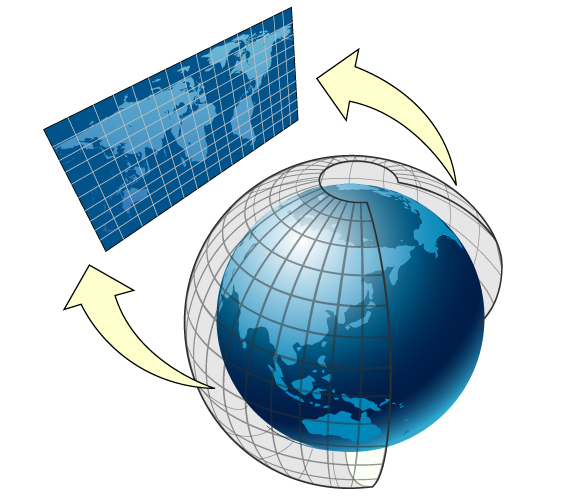
\includegraphics[width=0.4\textwidth]{sphere_to_cylinder}
\caption{Projection of a geographic coordinate system to a 2D flat map (source~\cite{projected})}
\label{figproject}
\end{figure}

To define a coordinate system, some parameters should be considered, such as the measurement framework (geographic  or planimetric), the unit of measurement (e.g. meter for the projected coordinate systems and decimal degrees for geographic coordinate systems), and the projection definition for the projected coordinate system.
%geographic (measuring spherical coordinates from Earth's center) or planimetric (projecting Earth's coordinates onto a two-dimensional planar surface)

In order to express the geospatial data by coordinate systems, various encodings have been developed by Open Geospatial Consortium (OGC)~\cite{ogc}, following different goals. OGC as an international consortium is the main reference to develop interface standards for geospatial content, services, data exchange, data communication, and data processing. Here, we introduce only a short list of common data representation standards which are related to our study.
%Additionally, there are terms for representing a geospatial data which a list of them is as follows,
\begin{itemize}

%\item Geometry: A geometry is a datatype to represent a location or a region. 
%TODO \item: encodings, baghiye subitem bashan (http://www.digitalpreservation.gov/formats/fdd/gis_fdd.shtml)

\item Geography Markup Language (GML): The XML-based standard encoding defined by OGC that serves as a modeling language to express geographical features in both spatial and non-spatial characteristic. It is used as an interchange format in internet data storage, exchange, transport, and transaction. The key to the effectiveness of GML is its capability in integrating all forms of geographic information. %TODO:ref az wikipedia!.
GML versions before Version 3.0 encode a set of 2D geometries, i.e. Point, LineString, and Polygon. GML 3.0 introduces Curve and Surface as new geometries, plus the support of geometries in 3D.

\item Keyhole Markup Language (KML)~\cite{kml}: An XML-based grammar to encode and represent the geographic data in an 3D earth viewer such as Google Earth, also on a 2D map like Google Maps. KML has been adopted as an international standard by OGC. The 3D geographic coordinates for each place are represented with longitude, latitude, and if available altitude. Coordinates are provided using the plain unprojected WGS84 longitude and latitude. The altitude could be omitted and assumed as $0$. KML mainly focuses on visualizations and expresses what and how to show the data. Code~\ref{kml} shows a sample data in KML. 
\vspace{10px}
\begin{fakeXML}[label=kml,caption=A simple KML example representing a Point]
<?xml version="1.0" encoding="UTF-8"?>
<kml xmlns="http://www.opengis.net/kml/2.2">
<Document>
<Placemark>
  <name>New York City</name>
  <description>New York City</description>
  <Point>
    <coordinates>-74.006393,40.714172,0</coordinates>
  </Point>
</Placemark>
</Document>
</kml>
\end{fakeXML} 
\vspace{10px}
\item Well-known Text (WKT): A text-based markup language to represent the vector geometries which supports a big range of objects like Geometry, Point, LineString, Curve, Polygon, Surface, curvePolygon, and multi-part geometries such as MultiPoint, MultiCurve, MultiSurface. Below are examples of Point, LineString, and Polygon represented in WKT: 
\begin{itemize}
\item Point: POINT (1 2)
\item LineString: LINESTRING (3 1, 1 3, 4 4)
\item Polygon: POLYGON ((3 1, 4 4, 5 4, 1 2, 3 1),
			(2 3, 3 3, 3 2, 2 3))
\end{itemize}
\item Well-known Binary (WKB): The binary representation of WKT data to be used in a database system.
\item GeoJSON~\cite{www/geojson}: A geospatial data encoding based on the JavaScript Object Notation (JSON). An object is represented by a set of name/value pairs. The whole data is encoded as text and no advanced numeric data types are employed. It is mainly used as a lightweight text format for data exchange. The default coordinate system in this standard is WGS84, however other systems could be defined. A sample point in GeoJSON is provided in Code~\ref{geojsonexa}:
\vspace{10px} 
\begin{fakeXML}[label=geojsonexa,caption=A simple GeoJSON example representing a Point]
{
    "type": "Point", 
    "coordinates": [30, 10]
}
\end{fakeXML}
\end{itemize}
\vspace{10px}

\subsection{Geospatial Data in Native XML Databases}
\label{s.geo-data-in-xml-data}
As a powerful platform-independent XML grammar introduced by the GIS community(OGC), GML plays an important role in spatial data modeling, integration, sharing, transmission, and exchange because of its flexibility in application schema, self-descriptive format, and rich data expression. Considering the XML-based structure of GML, it could be embedded and queried anywhere in the document, and be mixed with any other type of XML, images, etc. 
%TODO:In classic relational databases,... In XML native databases, geospatial data are handled ...

In addition to the general functions and features on the structure of GML data, geospatial concepts and requirements could be included in the native XML databases. To start with, the GML elements should be read and treated as geometries. Therefore, the string information is not enough to satisfy the geospatial features. The positions, locations, and relations between an arbitrary set of geometries raise some requirements regarding to the topics and definitions in related scientific fields like Geometry and Geoscience. For example, "What is the distance between two geometries?" or "Which geometries intersect a particular geometry?". Furthermore, there are features related to single geometries, such as the length and area of a geometry, the number of interior rings of a polygon, and the starting point of a line. These features can be provided as XQuery functions by a database system or XQuery processor and be mixed with standard XQuery, full-text, and other functions.
To this date, numerous ideas have been introduced for geospatial functionalities as well as indexing. Here we discuss some geospatial index structures and then we will have a look at some sample implementations in Section~\ref{s.dbs}.
%In order to investigate the related functionalities we start with the existing approaches in the indexing and the 

%Indeed in a database system the features related to a set of geometries are of more importance ...................
%TODO: We then present spatial comparisons as XQuery functions
%(similar to how the spatial operators are defined in spatial-enabled SQL
%engines) so they can be mixed with standard XQuery, full-text, etc.

%GML works nicely with XQuery and the indexing since it allows the engine to
%determine what to index, and it can be nested anywhere in an XML document.
%Furthermore, XQuery, with some additional functions to convert from the
%Well-Known Text/Binary formats used in other engines, is quite useful for
%building new GML on the fly, and parsing/validating existing GML.

\subsection{Geospatial Indexing}
\label{s.geospatial-index}
According to the survey of Chin et al~\cite{survey}, indexing has dramatic influences on data manipulation and storage. Conventional index types are not suitable for supporting geospatial data since it is very large and complex in structure and relations. Besides, the spatial queries differ from non-spatial queries in several important ways. For example, spatial queries include geometry data types and consider the spatial reletionships,e.g. containment, between the geometrirs. Additionally, the operators used for geospatial data retrieval are complicated and spatial orderings would be hard to define. An important reason which makes the traditional indices not appropriate is that indexing strategies will consider the spatial objects in one dimension and do not preserve the spatial proximity.

%As Chin et al~\cite{survey} has examined, As already has studied in several suryays, 
In order to fulfill the geospatial specialty and improve the data retrieval, a large number of spatial indexes has been introduced. The strength or weakness of an indexing approach mostly depends on the requirements, query types, and applications for which it is developed. 
The high percentage of these structures is based on the divide and conquer algorithm~\cite{divconquer}. 
In general, Chin et al~\cite{survey} have categorized all approaches to three different abstract classes:
\begin{itemize}
\item Object Mapping: Given a $k$-dimensional polygon with $n$ nodes, these approaches map this shape to a $kn$-dimensional or try to look at the shape of polygon as a single object in the original $k$-dimensional polygon.   
\item Object Duplication: These approaches keep different instances of an object in different spaces with the similar representations to take advantage of the properties of all these spaces. 
\item Object Bounding: Similar to the idea of Quad-tree~\cite{quadtree} and Marching cube~\cite{marchingcube} (an approach in Computer Graphics), 
these approaches enclose the polygon as accurate as possible by dividing the space in different ways. 
\end{itemize}

\begin{figure}
\centering
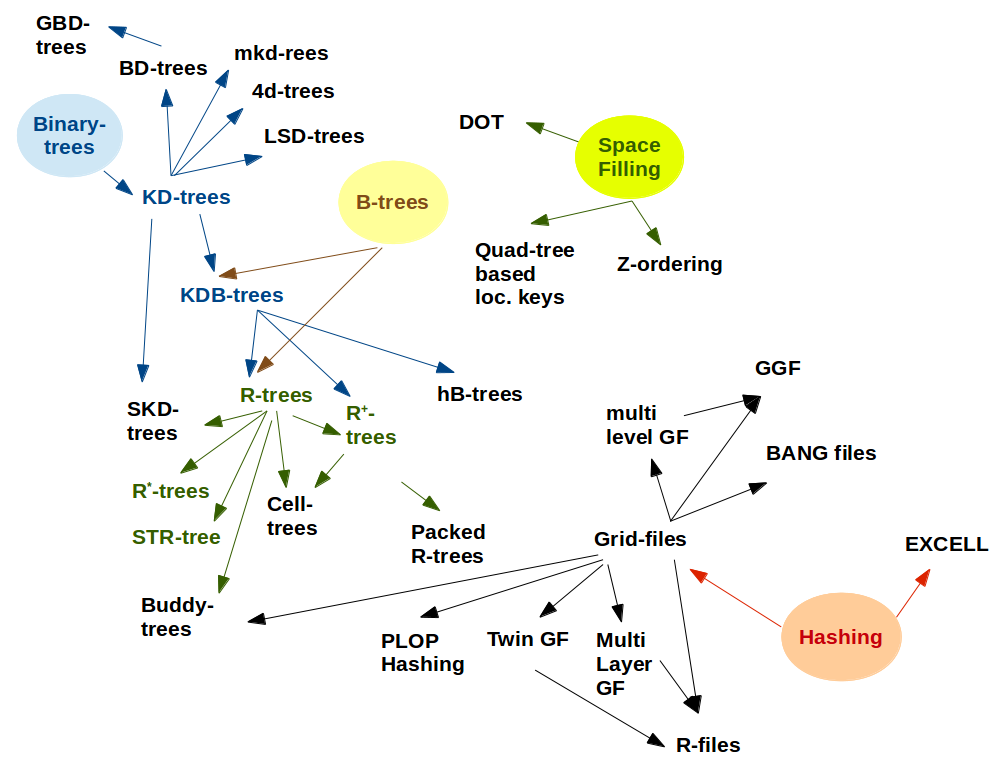
\includegraphics[width=0.9\textwidth]{Trees}
\caption{An overview of some important indexing structures developed over the years}
\label{trees}
\end{figure}

On the other hand, the index structures are mostly based on famous tree structures, like Binary-tree~\cite{binarytree}, B-tree~\cite{btree}, and Quad-tree. 
%To see how different approaches are developed based on these tree structres, 
%spatial indexes are introduced briefly based on these three famous data structures. 
To see how different approaches are developed based on these data structures, here we cover just a selective list of them. Figure~\ref{trees} visualizes the relation of some indexing structures which were developed over the years. An arrow from structure $A$ to $B$ means that $B$ is an extension of $A$. The colored circles also show the main categories of these
trees. In the upcoming sections, these structures are briefly explained:
Binary-tree based in Section~\ref{binary-tree-based}, 
B-tree based in Section~\ref{b-tree-based}, 
and Quad-tree in Section~\ref{quad-tree-based} from the space filling index structures.

\subsubsection{Binary-tree Based}
\label{binary-tree-based}
The indexes in this group are conceptually derived from the binary search tree by adopting and generalizing the idea of space partitioning. 
The KD-tree was the very first indexing structure of this kind introduced by Bentley~\cite{bently1975}. 
It is a generalization of the binary tree structure for organizing $k$-dimensional points. As Bentley~\cite{bently1975} explains, the basic idea for a 2D example is to alternatively split the area by $x$- and $y$-coordinate such that at each level the points are split half in left, half in right and half below, half above respectively. Generally, for every non-leaf nodes in the same level, there is a $k$-th dimension discriminator which defines the dimension along which the areas must be split to form the left and right subtrees. The split has to result in two subspaces such that the points in the left or below subspace have smaller value in the dimension which split happens, e.g. $X$, than the parent node and those in the right or above subspaces have greater values. More clearly, if the discriminator for a node is associated to the $i$-th dimension, after splitting a space along the $i$-dimension all $i$-th attribute of the left subtrees nodes have smaller value than the $i$-th attribute of this node and all the right subtree nodes have the greater $i$-th attribute. 

Figure~\ref{figkdtree} shows the representation of some sample data and the corresponding KD-tree. As it can be seen, according to the discriminator $x$ in the first level, nodes $B, C, D$ in the left subtree of $A$ have a smaller $x$ value and nodes $E, F$ in the right subtree have a greater $x$ value. In the next level that the discriminator is $y$, the same consequently happens for $y$ values. For example, node $C$ which is in the subspace half below $B$, has a smaller $y$ value.

The KD-tree as an important search structure, has been widely used and studied~\cite{ilprints723}. With a simple implementation, it works effectively for range queries since they are formed by splitting the space by planes orthogonal to axis. The balanced KD-tree is also effective in searching the Nearest Neighbour in 2D which plays critical roles in database retrievals, classification problems, and clustering problems together with other reange queries. However, some variants have been introduced to allow for better performance in clustering, searching, storage efficiency,  
and balancing, especially in higher dimensions. We discuss some of these variants in the followings.

\begin{figure}
\centering
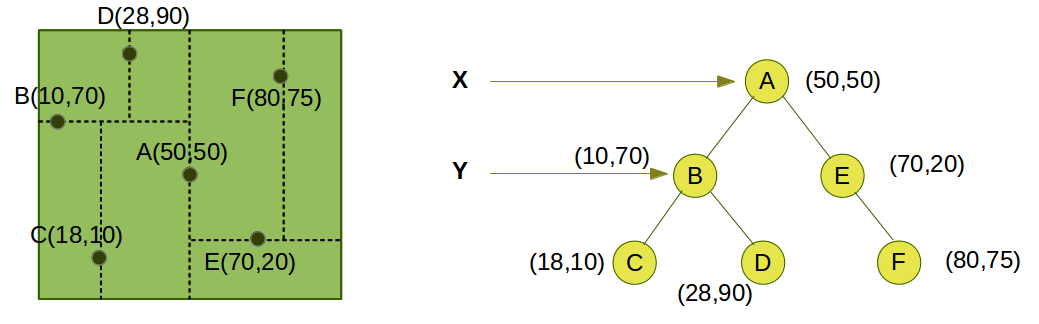
\includegraphics[width=0.8\textwidth]{kd-Tree}
\caption{A representation of KD-tree}
\label{figkdtree}
\end{figure}


\textbf{Non-homogeneous KD-tree.}
A complication arises when an item is deleted from the KD-tree and a node from the subtrees must be replaced. This complication comes from the discriminator in that level. After the deletion, either the node with the smallest value in the right subtree should be replaced or the node with the biggest value in the left subtree. 

The Non-homogeneous KD-tree~\cite{nonhomkdtree} was proposed to make the process of deletion cheaper. The major alteration to build this structure is that the partitioning is not always on different dimensions cyclically. Instead, the dimension including more range queries is selected to be the discriminator in each level. For example, if the discriminator at the first level is $x$, at the second level it can be $x$ again instead of $y$ in a two-dimensional KD-tree. 
The partitioning in this tree can happen in an arbitrary hyperplane like a line in 2D in contrast to KD-tree that a data point is always chosen for partitioning. In this partitioning, almost-balanced subplanes are desired.
 
\textbf{KDB-tree.} Another issue to be discussed here is storage efficiency of indexing.
Since the size of indexing can grow fast enough to fill a huge chunk of main memory, most of the index structure must be stored necessarily on disk while being used.
To make efficient use of the secondary memory, the KDB-tree~\cite{kdbtree} is proposed to provide the search efficiency of a balanced KD-tree together with the optimized storage access taken from the B-tree. It partitions the areas similar to the KD-tree and stores each node as a page similar to the B-tree. Pages exist in two types, 
%as takes advantage of the paging technique~\cite{bintreepaging} together with the balanced structure of KD-tree. 
%The KDB-tree uses a space partitioning method such that the partitions do not overlap each other. ????
%Although this space partitioning is similar to the KD-tree, more than one nodes can be stored together as pages. ????
%Then, these pages are stored as nodes of KD-tree.
%The KDB-tree has two basic structures:
region and point pages. A region page as an internal node contains a description of the bounding region enclosing its children and reference to the children. 
%\todo the figure is not correct.
A point page as a leaf node carries the object identifiers. Therefore, different pages are kept in different parts of memory instead of a huge chunk. 

As a property of the KDB-tree structure, the regions in every region page are disjoint and their union is the parent region. %Moreover, the union of regions in a child region page is the parent region. 
Similarly, all points in a point page as a child of a region are placed necessarily in that region.
As shown in Figure~\ref{figkdbtree}, $D$, $E$, $F$, and $G$ subspaces are disjoint and shape together the region $A$ as the parent node. Here, the black small points in the leaf nodes are representing the points belonging to a page. Also, the hatched areas in each node are the regions which are not included in the page of that node. 
As Robinson~\cite{kdbtree} states, the KDB-tree represents a more efficient search structure for large multi-dimensional dynamic structures with optimized storage utilization. It should be mentioned that there is a trade-off between being height-balanced and storage efficiency. Then, the storage efficiency can be even poorer in some cases.

\begin{figure}
\centering
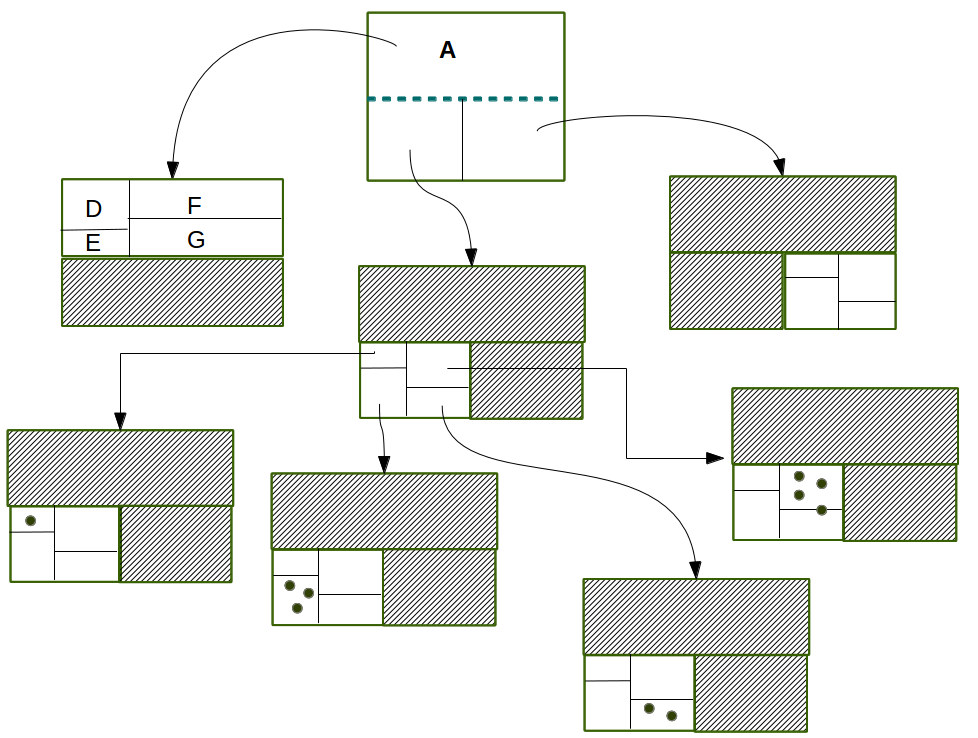
\includegraphics[width=0.8\textwidth]{kdbtree}
\caption{A representation of KDB-tree(created based on~\cite{kdbtree})}
\label{figkdbtree}
\end{figure}

\textbf{HB-tree.} 
Splitting the region nodes is inevitable for keeping the balance of KDB-tree during the modification processes. This splitting is done by intersecting the data space with a plane. This intersection does not always cross the actual borders of current subregions. Then, new subspaces would be produced. This means that that splitting can propagate to the children, resulting in more and more sparse nodes in lower levels. The HB-tree (holey brick B-tree)~\cite{hbtree1} as a multi-attribute index structure is proposed to solve this problem. This structure allows data spaces to be divided along more than one dimension such that rectangular regions inside that space can be shaped, called holes.
%It permits rectagular holes inside a data space by partitioning along pieces of several dimensions. 
This gives more flexibility in partitioning and serves as a solution for the cases in which partitioning a region along one entire dimension forces splitting of the children subregion. 

The HB-tree also helps to distribute the objects in subspaces more evenly when it is not possible by cutting across one dimension. Figure~\ref{hbtree} illustrates an example at which partitioning along one dimension in~\ref{hbsplita} results in uneven division of data while two-dimensional split in~\ref{hbsplitb} divides the objects more evenly.

\begin{figure}
\centering
\subfigure[Single-dimensional split of data points]{
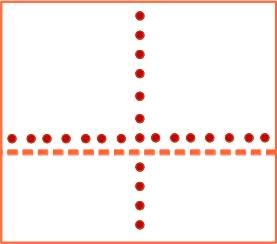
\includegraphics[width=0.22\textwidth,height=0.12\textheight]{hbtree1}
%\caption{R-tree structure}
\label{hbsplita}
}
\centering
\subfigure[Two-dimensional split of data points]{
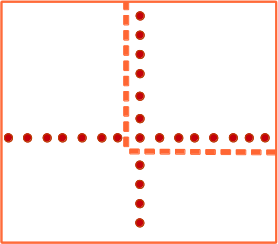
\includegraphics[width=0.22\textwidth,height=0.12\textheight]{hbtree2}
%\caption{R-tree}
\label{hbsplitb}
}
\caption{Partitioning of data space in HB-tree (based on~\cite{tree-basedindexes})}
\label{hbtree}
\end{figure}

To represent the holey regions, the HB-tree uses the KD-tree within internal nodes to organize the information about the lower levels. It means that a more complex data structure is required to represent a node. In addition, it might happen that a region is referenced by more than one leaf of the KD-tree in internal nodes of the HB-tree, such as node $G$ in Figure~\ref{fighbtree}. As it can be seen in this Figure, splitting along $y$ on the third level results in dividing into two subtrees, one having $1/3$ and the other $2/3$ of the nodes. To achieve this, the subtree with node $x_2$ shows the split along $x$ in the next level and therefore duplicates $G$ in both right and left subtrees. The subtrees with root nodes $x_1$, $x_2$, $y_3$, and $y_5$ are extracted to show $F$ and $C$ regions.
%, since part of it is below and the other part is above $y_5$. Obviously, $F$ is in the left subtree as the lower region. Then, in the next level, partitioning along $x$ dimnesion puts $G$ in left and $F$ in right. This means, to represent the "hole"

\begin{figure}
\centering
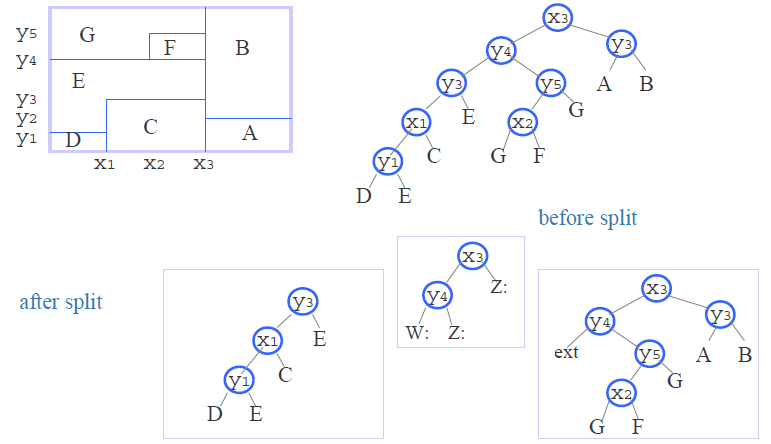
\includegraphics[width=0.65\textwidth,height=0.2\textheight]{hbtree}
\caption{A representation of HB-tree (source~\cite{hbtree1})}
\label{fighbtree}
\end{figure}

%In HB-tree leaf nodes are called \textit{data nodes} and internal nodes are \textit{index nodes}. 
%Index nodes  
%A data space can be non-rectangular and space representation in internal nodes is by KD-trees. The leaf nodes are known as data nodes and the internal node as index nodes. An index node data space is a union of its child node subspaces which are obtained through KD-tree recursive partitioning.
As Lomet and Salzberg~\cite{hbtree1} states, removing the sparse nodes of the KDB-tree gives better search and insert performance and decent space utilization in the HB-tree. Nevertheless, expensive deletion and splitting as a result of complex structure, and multiple references to a data node that may lead to more than one traversal of a path are the trade-off.

\textbf{Matsuyama's KD-tree.} Since KD-trees are designed as a point access method, the variant structure introduced by Matsuyama et al~\cite{matsuyama} is suitable for non-point objects via adding an extensive duplication strategy. In order to achieve this, a data page is associated to each leaf node containing pointer to the objects. The pointers refer to objects either totally or partially included in the data space. Those objects that overlap several unpartitioned spaces will be referenced in all corresponding pages. As mentioned in~\cite{survey}, this structure is not appropriate for data with large objects due to duplication.

\textbf{4D-tree.} Another extension of the KD-tree to make it useful for two-dimensional rectangular objects is the 4D-tree~\cite{4dtree}. This data structure maps objects into four-dimensional points which are indexed in the KD-tree. It means that a rectangle $(x‍‍_1, y_1)$, $(x_2, y_2)$ is considered as the point $(x‍‍_1, y_1, x_2, y_2)$. Similar to the KD-tree, the discriminator in each level is chosen repeatedly from the set $(x‍‍_1, y_1, x_2, y_2)$. For each node, a discriminator, a discriminator value, and pointers to two children are stored. 
For a region search $(qx_1, qx_2, qy_1, qy_2)$, depending on the discriminator, the result of one of the following operators,
$$x_1 \leq qx_2, \quad x_2 \geq qx_1, \quad y_1 \leq qy_2, \quad y_2 \geq qy_1,$$ 
determines which subtree (or both) has to be searched.
The major problem of this approach is the high cost of its intersection search when the query needs propagating in both subtrees. 


\textbf{SKD-tree.} The Spatial KD-Tree (SKD-tree)~\cite{skdtree} alters the KD-tree such that the object duplication and object mapping is avoided. Similar to the 4D-tree, it was proposed to handle non-point spatial objects since they may extend in more than one subspace in the KD-tree. To prevent those objects to be divided and referenced multiple times, the SKD-tree defines a virtual subspace for each subspace produced in the KD-tree. Each virtual subspace determines the bounding area of all objects with the centroid inside the original subspaces. It means that even though an object is not totally contained in the original subspace, it can be contained in the corresponding virtual subspace. More clearly, the objects will be placed in subspaces based on their centroid. Therefore, each node has the following parts~\cite{skdtreebook},
\begin{itemize}
\item Pointers to two children
\item The level discriminator
\item The level discriminator value
\item The maximum and minimum values of the left and right subtree objects respectively in the dimension that the level discriminator belongs to.
\end{itemize}    
As Chin et al~\cite{survey} state, the SKD-tree directory is stored in secondary memory. Figure~\ref{figskdtree} shows an example of a data set and the space partitioning together with the corresponding SKD-tree. Figure~\ref{skdtree2} illustrates the way that minimum and maximum boundaries of each space are determined to shape a virtual subspace. In this example, the discriminator for the root node is $x$ with the value of $x_6$.
The maximum boundary of the rectangle $r_3$ is $x_7$ which defines the maximum boundary of the left virtual subspace. Correspondingly, the minimum boundary of the right subspace is $x_5$, which is the right boundary of rectangle $r_8$. Figure~\ref{skdtree1} shows the tree directory of this sample data.
\begin{figure}
\centering
\subfigure[Space partiotioning in the SKD-tree]{
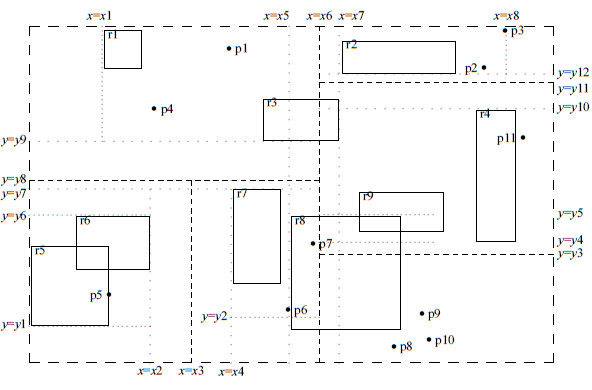
\includegraphics[width=0.5\textwidth,height=0.19\textheight]{skdtree2}
%\caption{}
\label{skdtree2}
}
\centering
\subfigure[A 2D directory of the SKD-tree]{
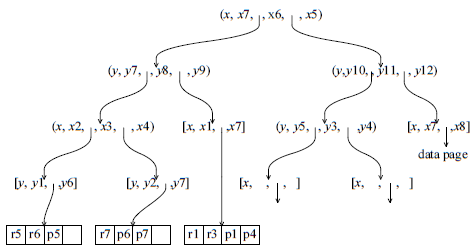
\includegraphics[width=0.5\textwidth,height=0.19\textheight]{skdtree1}
%\caption{}
\label{skdtree1}
}
\caption{An example of the SKD-tree structure (source~\cite{survey})}
\label{figskdtree}
\end{figure}
The SKD-tree is at the advantage when the virtual subspace may bound the objects tighter than the partitioning line. In such cases, the intersection search cuts the search space efficiently. The containment search is directly supported in this structure and is useful to operators, like \textit{within} and \textit{contain}, since all objects, which are not contained totally in the query region, are ignored.
As the SKD-tree is memory-based, not disk-based, it is not suitable for very large databases.

%Main memory storage of the index trees are mostly a problem, since it is too big to be placed there  [survay]. Hence, the storage has to be done into disk space. Using binary search tree paging techniques [CeS82 survay] or tree organization of B-trees [BaM72 survay] to store the kd-Tree proposes new indexing structures.
%Using properties of both kd-tree and B-tree [reference], the KDB-tree rebuilds the kd-tree to improve some inefficiencies of it.  It means that benefits of the balanced kd-trees and the I/O efficiency of B-trees are together. It uses the disk space to bring the kd-tree on disk. 

 


\subsubsection{B-tree based Indexing Technique}
\label{b-tree-based}
The B-tree is used extensively in databases due to its flexibility and ability to handle a large amount of data. However, it is not designed for data in multi-dimensional spaces. Therefore, it is not suitable for spatial searches like other classical one-dimensional index structures. Frequent queries in geospatial applications, such as finding the all places within $20 km$ of a point, make it important to find the objects according to their spatial location in a space. Regarding the utility of B-tree, a variety of index structures have been developed based on its structure and focusing to meet the spatial requirements. In the followings we discuss some of these structures.

\textbf{R-tree.} The R-tree~\cite{rtree}, as one of the spatial indexing structures, extends the B-tree by adding support for multi-dimensional data. It also inherits the height balance from the B-tree. This structure is designed based on the idea of grouping the neighbouring objects and representing them with their minimum bounding rectangle (MBR). The idea minimizes the visiting area in spatial queries. Shapes and objects are described in leaf nodes by rectangles containing a single object. Each non-leaf node in higher levels is the smallest bounding rectangle spatially containing its children, either the rectangles or objects. The root node with at least two children is the biggest minimum bounding rectangle which spatially contains the whole objects. Figure~\ref{rtree} depicts how an R-tree is built for a spatial data set. Figure~\ref{rtreebox} illustrates the minimum bounding rectangles calculated for different levels
% from those which contain the single objects to those containing the whole area. 
and the corresponding R-tree is shown in Figure~\ref{rtreestruct}.
As this structure is designed for disk storage, the leaf nodes in Figure~\ref{rtreestruct} point to the data tuples on disk.
%More clearly, the leaf nodes in R-tree are the actual shapes while
%other nodes are minimum bounding boxes of the actual geospatial data. Here, 
%the actual bounding boxes have the dimension of the data.



\begin{figure}
\centering
\subfigure[Minimum bounding rectangles of an object set to build the R-tree]{
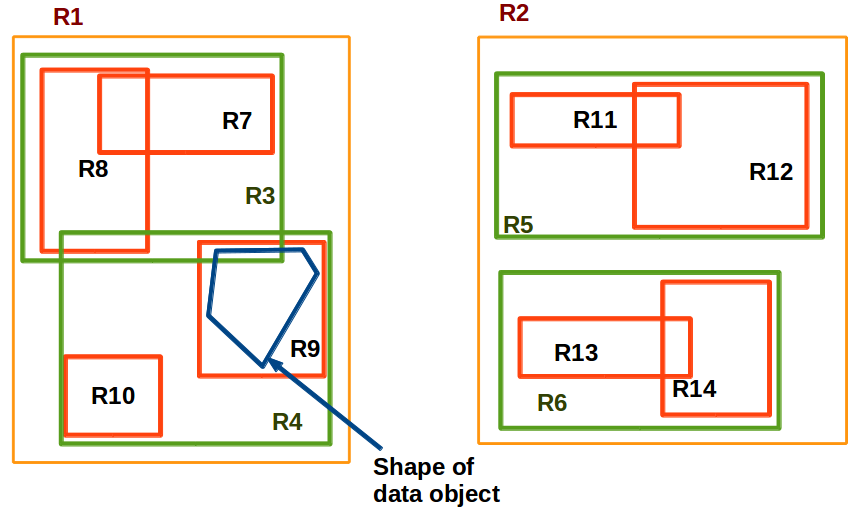
\includegraphics[width=0.47\textwidth,height=0.17\textheight]{Rtree-box}
%\caption{R-tree structure}
\label{rtreebox}
}
\centering
\subfigure[R-tree structure]{
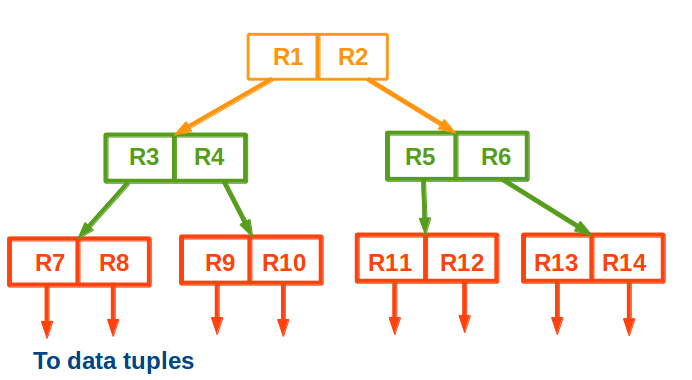
\includegraphics[width=0.47\textwidth,height=0.17\textheight]{Rtree}
%\caption{R-tree}
\label{rtreestruct}
}
\caption{A sample of R-tree creation for a set of spatial objects in 2D}
\label{rtree}
\end{figure}

According to Chin et al~\cite{survey}, the operations on the R-tree 
are basically the same as in the B-tree. The only difference is that the 
whole operations have to be done on bounding rectangles.
Also, the order used in the element placement in B-tree
is the set inclusion order on bounding rectangles and shapes in leaf nodes. 

Partitioning the area with MBRs is the challenging point of the R-tree. Each split algorithm, generates different partitions such that the R-tree structure may differ for each of them. Since the rectangles are areas to be investigated in spatial calculations, minimizing both their coverage area and overlapping is crucial to its performance. Therefore, splittings should result in the minimum total area of rectangles and minimum overlapping of each two rectangles. 
Achieving these goals largely depends on the splitting algorithm chosen for defining the bounding rectangles. Figure~\ref{rtreesplit} illustrates this point by two different splits. Total coverage area of the "Bad split" case in this sample is larger than the "Good split" and this will lead to unnecessary investigation of empty spaces.

\begin{figure}
\centering
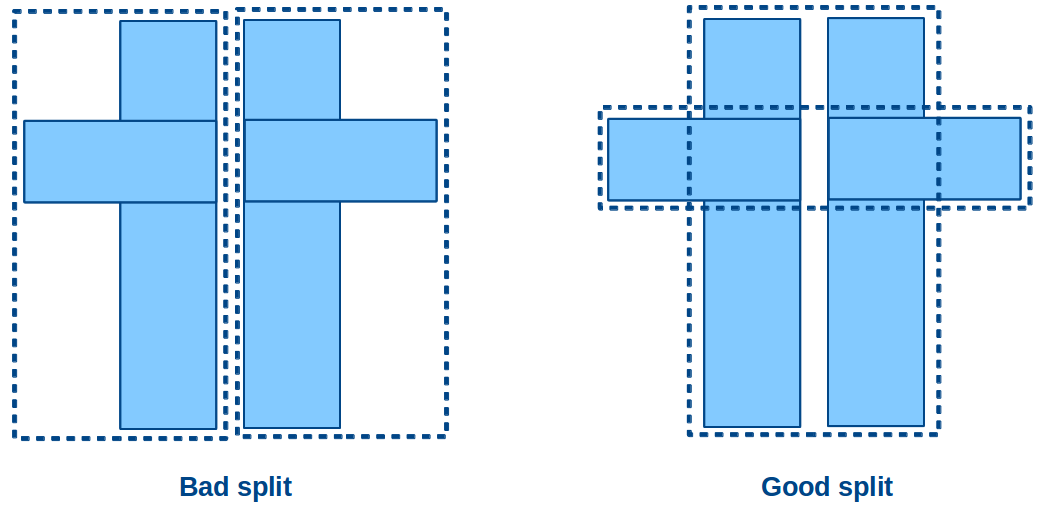
\includegraphics[width=0.5\textwidth,height=0.17\textheight]{R-treeMBR}
\caption{Two different split strategies in the R-tree (created based on~\cite{rtree})}
\label{rtreesplit}
\end{figure}

As mentioned before, the idea of bounding rectangles helps to decide which parts of the tree have to be visited in search queries, such as intersection, overlapping, and containment. In fact, the following steps are taken to run such queries,
\begin{enumerate}
\item Filtering: This step selects those rectangles which overlap the query area.
\item Spatial Operation: The requested spatial operation is applied on the selected rectangles from Step $1$. 
\item Step $2$ continues until it reaches those rectangles containing single objects. 
\item The selected objects are checked against the query operation. 
\end{enumerate}
Figure~\ref{rtreequery} depicts how an intersection query is done on the R-tree and how the rectangles are chosen to be included in calculations. In this example, the rectangles $R_2$, $R_5$, $R_6$, $R_{12}$, and $R_{14}$ are selected to be checked while the other areas remain untouched. At the end $R_{12}$ and $R_{14}$ are selected as rectangles containing the final results.

\begin{figure}
\centering
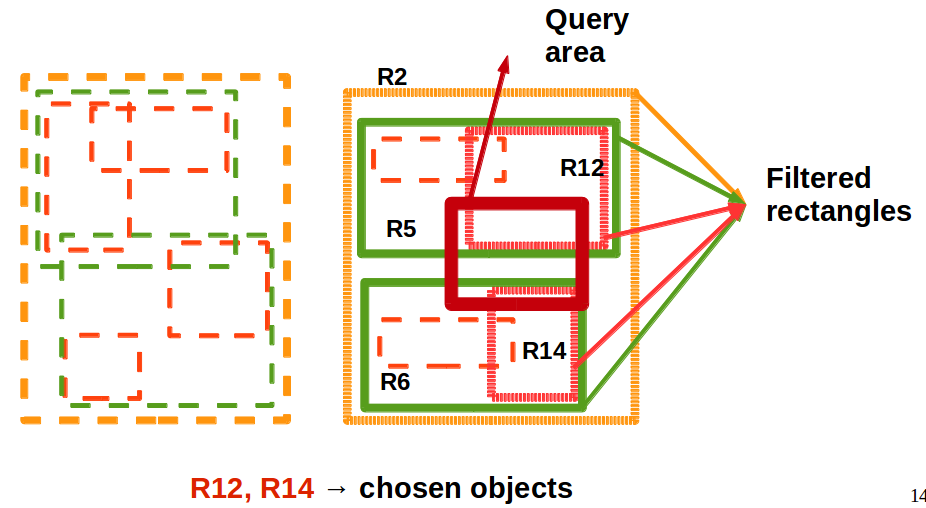
\includegraphics[width=0.6\textwidth,height=0.2\textheight]{Rtree-query}
\caption{Querying the R-tree}
\label{rtreequery}
\end{figure}

The R-tree benefits from the highly balanced structure and organizes the data in pages. This structure is designed for secondary storage and most of implementations often keep the inner nodes in main memory while the leaves are loaded from disk. It yields good performance in low-dimensional spaces. Generally, this structure is common indexing technique for efficient execution of multi-dimensional queries on both point and extended spatial data. However, there are two main disadvantages according to Manolopoulos et al~\cite{Manolopoulos:2005}, which motivate to revise the structure towards more efficient variations. First, point-location queries may lead to multiple path navigations in the tree leading to declined performance, especially when MBRs overlapping are considerable. Second, investigating empty spaces of large rectangles which have significant overlaps, deteriorates the performance. Here, we briefly explain some of the most important variations of the R-tree to see how they alter the algorithm to circumvent the disadvantages. The improvements for R-trees can be grouped into two groups with distince objectives, \textit{dynamic} and \textit{static}. The dynamic variants effectively handle insertions and deletions on an existing tree while the static ones must be known in advance and build an efficient tree from scratch. 


\textbf{$\boldsymbol{R^+}$-tree.}
The $R^+$-tree~\cite{Sellis:rplustree} is introduced as a compromise between the R-tree and KDB-tree. In simple words, the $R^+$-tree avoids overlapping of internal nodes (rectangles) at the same level of tree. To obtain this, objects will be inserted in more than one leaf if necessary. Figure~\ref{r+tree} shows an example of an $R^+$-tree together with its corresponding planar representation. As it can be seen, the node $e$ which is partially contained in both rectangles $C$ and $B$, is referenced twice in the leaf nodes.

%It has just some difference:
%Nodes of an R+-tree are not guaranteed to be at least half filled.
% The entries of any intermediate (internal) node do not overlap.
% An object identifier may be stored in more than one leaf node.

\begin{figure}
\centering
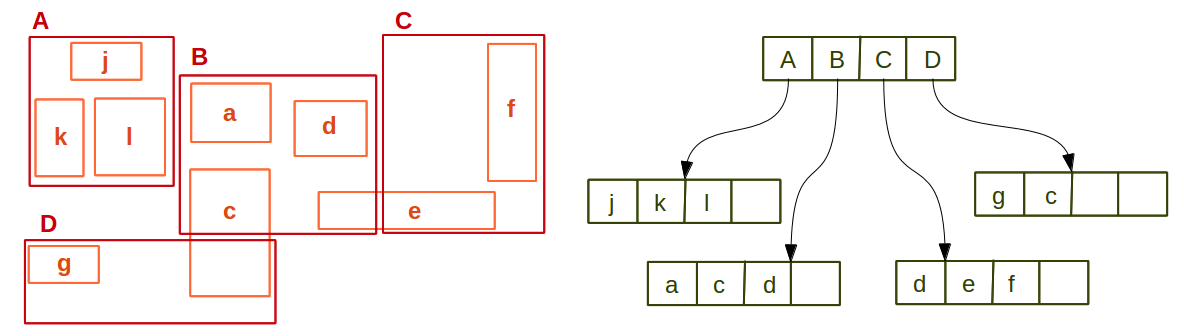
\includegraphics[width=0.9\textwidth]{r+tree}
\caption{An {$R^+$-tree} example}
\label{r+tree}
\end{figure}

With the changes made in the structure, the $R^+$-tree is at some advantages. Performance for points
queries is better due to the absence of overlapping. Instead of several paths, a single path is traversed. Consequently, fewer nodes are visited in point queries. On the other hand, there are some disadvantages. 
%The duplication of the objects avoids overlapping and consequently leads to less path traversals in point queries. 
%On the other hand there is some disadvantages: 
The {$R^+$-tree} might be bigger than the R-tree as a result of duplicating rectangles. Additionally, construction and maintenance are more complex in the {$R^+$-tree}. Furthermore, The increased complexity of the deletion algorithm is another drawback of the approach of avoiding overlaps. 
According to G{\"u}nther~\cite{efficientstruct}, there is another problem in the {$R^+$-tree} algorithm which could happen in some insertions. It happens when the covering rectangles do not allow each other to expand in order to include the inserted object. As a result, the so-called \textit{dead spaces} are produced in the current structure that cannot be covered. It means that if a new object places in those regions, it cannot be fully covered. To cover the uncovered areas, one or more rectangles have to be split and this leads to splitting of some children as well. This case degrades the storage efficiency. %However, Chin et al~\cite{survey} state that {$R^+$-tree} performs generally better for smaller objects and slightly worse for larger objects. 
However, the overall performance of this structure is improved as a result of e absence of overlap between MBRs in internal nodes~\cite{Papadopoulos2010}.
%In performance study, in the comparison between R-trees and R+-trees, it is found that the R+-tree requires much more splits, especially for large data objects, but lesser splits for smaller data objects. 

\textbf{The Cell Tree.}
To avoid the overlapping problem of R-tree and \textit{dead spaces} in the $R^+$-tree, the cell tree~\cite{celltree} was introduced. Partitions in this tree may be convex polyhedra as bounding polygons, instead of rectangles, such that the partitions do not overlap. 
Since some spatial objects are shaped irregularly, this method gives a better approximation of them.
For example, the internal nodes in Figure~\ref{figcelltree} are polygons. 
\begin{figure}
\centering
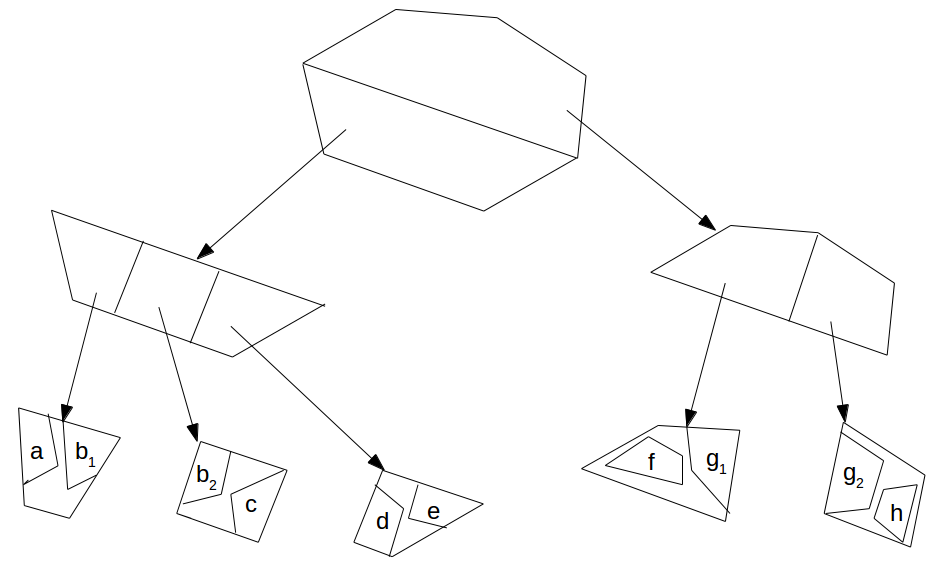
\includegraphics[width=0.7\textwidth]{CellTree}
\caption{An Example of a cell tree (source~\cite{survey})}
\label{figcelltree}
\end{figure} 

Similar to the $R^+$-tree, objects may be stored in more than one leaf if necessary. This could lead to a division of new objects in order to place them in bounding polygons that do not overlap. 
As an instance, the object $b$ in Figure~\ref{figcelltree} is contained in two different leaf nodes as $b_1$ and $b_2$.
This will be more serious in populated databases. The solution proposed by Chin et al~\cite{survey} improves storage efficiency, but does not give significant query performance. 

\textbf{$\boldsymbol{R^*}$-tree.}
In order to achieve better performance, $R^*$-tree~\cite{rstartree} goes beyond the MBR area minimization by trying the following criteria, as Manolopoulos et al~\cite{Manolopoulos:2005} explains:
\begin{itemize}
\item Minimizing the covered area by MBRs to minimize the dead spaces which leads to fewer paths needed to be traversed in queries. 
\item Minimizing the MBRs overlapping to reduce the paths which must be followed by queries.
\item Minimizing the MBR margins to shape squarish rectangles which improve the performance of queries with large quadratic shapes.
\item Maximizing of storage utilization. 
\end{itemize}
In fact, unlike the R-tree which determines the MBRs according to their area, the $R^*$-tree determines them based on their area, margins of space, and overlaps with other MBRs. Additionally, \textit{Forced Reinsertion} is a key concept in this algorithm which deletes and reinserts elements of a full node to prevent splits.
To find the best combination of the criteria, it is necessary to implement an optimized approach. This is important since the criteria can conflict sometimes. The optimization is obtained with a revised node split algorithm and also forced reinsertion which finds a better place for a node than its original place. This structure results in the following performance improvements,
\begin{itemize}
\item More rectangular pages produced by the revised split algorithm are better for many applications.
\item Better performance is gained through the reinsertion method, however it increases the complication.
\end{itemize}
As expressed by Beckmann et al~\cite{rstartree}, the efficiency of $R^*$-tree is generally better than R-tree and some other variants, although it has slightly higher implementation cost than the R-tree.
% $R^*$-tree is found to be more efficient than some other variants,
%and R-tree using linear splitting algorithm is substantially less efficient than the one with quadratic splitting algorithm. 
%In general, $R^*$-tree is an improvement over the R-tree at the expense of more expensive insertion.

%This structure tries to reduce overlaps between directory rectangles and the area covered by a rectangle, in order to make better performance, since minimum overlaps leads to less number of branches to be traversed in queries and minimum coverage helps to decide on the paths to traverse on higher levels. 
%R*-Tree does these optimizations with revised node split and also forced insertion which finds a better place for a node that its original place. In R-Tree insertion-build structure is highly suboptimal and insertion and deletion could improves the R-Tree dramatically.
%(Using the idea of reinsertion of the R-tree, Beckmann et al proposed a reinsertion algorithm when a node overflows. The reinsertion sorts the entries in decreasing order of the distance between the centroids of the rectangle and the covering rectangle and reinserts the first p (variable for tuning) entries. In some cases, the entries are reinserted back into the same node and hence a split is eventually necessary. The reinsertion will no doubt increase the storage utilization; but it can be fairly expensive when the tree is large. 
%The R*-tree is found to be more efficient than some other variants, and the R-tree using linear splitting algorithm is substantially less efficient than the one with quadratic splitting algorithm. In general, the R*-tree is an improvement over the R-tree at the expense of more expensive insertion.)

%\textbf{The Buddy Tree.}
%(In comparison to previously proposed tree structures such as the K-D-B-tree, the buddy-tree guarantees a more efficient dynamic behavior.Moreover, indirect splits which cause low storage utilization and high insertion costs in the K-D-B-tree, are completely avoided. This structure is 
%It avoids the downward splitting of the K-DB-tree, the overlapping problem of the R-tree and the dependency of structures upon the insertion of data. The buddy-tree generalizes the buddy system of the grid-file to organize correlated data efficiently, by bounding the data points tightly using the bounding rectangle concepts of the R-tree and organize the directory as in the R-tree. Like grid-files, the non-zero sized data have to be mapped into higher dimension.
%An important feature of the buddy-tree is that it does not partition empty data space. Therefore queries, such as partial match queries, where the query region intersects with empty data space, can be performed much faster than by conventional structures partitioning the complete data space.
%The following summarizes the design properties of the buddy-tree:
%empty data space is not partitioned insertion and deletion of a record is restricted to
%exactly one path no overflow pages directory grows linear in the number of records
%performance is basicly independent of the sequence of
%insertions efficient behavior for insertions and deletions very high fan out of the directory nodes)

\textbf{X-tree.}
The X-tree, proposed by Berchtold et al~\cite{xtree}, is another extension to support high-dimensional data processing. X-trees focus on the prevention of MBR overlappings in order to minimize the amount of paths that have to be traversed. Unlike $R^+$-tree, this approach does not split a data region. Instead, it uses a more complex algorithm by analyzing the size of overlap occurred for each split. Then, it decides on choosing the minimum overlapping or creating a new kind of node, called \textit{supernode}. \textit{Supernode} refers to internal nodes containing more data values and pointers than the maximum capacity of normal nodes. In fact, supernodes are constructed to contain the extra entries when there is no good split, particularly in high-dimensional spaces which overlapping becomes a serious problem. Figure~\ref{figxtree} shows the supernodes in gray which are extended to contain six node links instead of three in normal nodes. This will help to decrease the tree levels and consequently improves the efficiency of search queries.

\begin{figure}
\centering
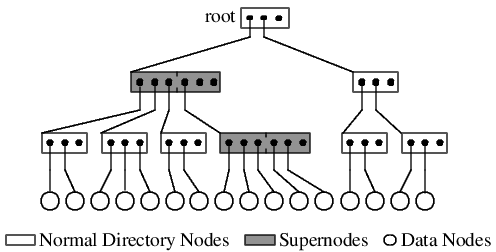
\includegraphics[width=0.7\textwidth]{xtree}
\caption{Structure of the X-tree (source:~\cite{xtree})}
\label{figxtree}
\end{figure}

\textbf{R-tree with packing algorithms.}
Suppose all the required data is available or at least does not change frequently when the tree is going to be built. For instance, in census and cartographic and environmental data insertions ade deletions rarely or even never happens. 
For such applications, constructing an optimal structure should be focused with regards to some tree characteristics, such as maximizing the storage utilization and minimizing the storage overhead, coverages, and overlaps in the R-tree. The methods to build such an R-tree contain a preprocessing step and are known as \textit{packing} or \textit{bulk-loading}. 
The packed R-tree, proposed by Roussopoulos and Leifker~\cite{packedrtree, packedrtree2}, is one of the statically constructed R-trees which has this preprocessing step. This early effort simply suggests to order the objects based on a criterion, like ascending $X$ coordinate. Then, to build the tree, the object with the minimum value of in the ordered set is chosen to find its \textit{M nearest objects}. Here, $M$ is the maximum number of objects that are allowed in a page. These nearest objects form a node. The bounding boxes of these objects also shape the higher nodes. This step is repeated until the whole objects are assigned to a node and the tree is completed up to the root.

The Hilbert Packed R-tree is another method to construct a static R-tree using the packing algorithm by Kamel and Faloutsos~\cite{hilbert-rtree}. This method which has a full space utilization, proposes sorting the objects based on their Hilbert value of their center and then inserting them into the tree.
The packed R-trees could be created with other packing algorithms. In the following, another packing algorithm is described which we will use to create a static index structure.
%To achieve the best minimization of covering rectangles, 
%The main objective of this algorithm is to reduce the storage space, the coverage and overlap of rectangles, in order to improve the search efficiency.

\textbf{Sort-Tile-Recursive (STR).} Sort-Tile-Recursive (STR)~\cite{strtree} is the state-of-the-art packing algorithm to build a static R-tree. As we discussed before, a dynamic R-tree may not give always the best structure, in addition to the high load time and suboptimal space utilization. Therefore, static creation in cases at which the data does not change frequently, is advantageous. The so-called STR-tree approach sorts the rectangles by their $X$ coordinate and then places them into $\sqrt{r/n}$ vertical tiles such that the number of rectangles in each tile is $\sqrt{r/n}$. Here, $r$ is the number of total rectangles and $n$ is the maximum number of rectangles that can be inserted in each node. Then, the rectangles are sorted by $Y$ coordinates. At the end, the rectangles are inserted in tree nodes in sorted order.
As declared in~\cite{strtree}, this structure improves space utilization and query performance as well as the other packing structures. However, in case of data modification the whole structure must be rebuilt.

\subsubsection{Quad-tree}
\label{quad-tree-based}
Another general category of indexing structures is the space filling structures which is studied in Jagadish~\cite{spacefilling}.
Among this category, we present the Quad-tree~\cite{quadtree}, which is mostly used in geospatial indexing. Quad-trees are based on the principle of recursive decomposition. The goal of this tree is to design a structure in main memory, often for two-dimensional data. 

In fact, Quad-tree is a class of tree structures in which the common structure, called \textit{region Quad-tree}, is based on the subdivision into four equal-sized quadrants. It means that each internal node has four children. The spaces may have rectangular or any arbitrary shape. The leaf nodes represent the corresponding data contained in a region. The space is divided more and more in the regions in which the data is more dense. As a result, this structure is very efficient for sparse data.
Several variants of Quad-tree have been introduced to obtain an optimized structure such as Quad-CIF-tree~\cite{quadcif}, MX Quad-tree~\cite{quadmx}, and a combination of both, MX-CIF Quad-tree. However, most of them satisfy the common properties, are easy to implement and provide good performance for two-dimensional data.
It should be mentioned that the performance is not always good since the tree might not be balanced and main memory maintenance of the structure is tricky due to the poor I/O throughput. Also, as we discussed, this data structure is basically designed for two dimensional data. Then, another similar idea should be taken for higher dimensions.
%It is organized in a way similar to the region quad-tree. A region is recursively partitioned until the resulting quadrants do not contain any rectangle. During the subdivision, all rectangles that intersect with either of the two partitioning lines are associated with the partitioning lines. The rectangles that are associated with a quadrant must not belong to any ancestor quadrant. It is assumed that no two rectangles overlap.
%\textbf{Cell Methods based on Dynamic Hashing}
\subsection{Summary}
\label{indexsummary}
In this section, we mainly explained some important spatial indexing trees which are widely studied in the literature. Indeed, there is a huge number of indexing structures introduced in various sources over this area. Also, these structures are categorized differently in each source. However an extensive research on indexing trees was not our focus, we tried to cover a set of leading ones as an introduction in developing a proper index structure in BaseX. As mentioned before, choosing an index depends on the characterisitc of system and also the functionalities that the system provides. Of course the spatial characteristic of data should be considered as well. 
Regarding the discussion in this section, there is no optimum indexing structure for any type of data and requirements. Based on the application, each structure has own pros and cons. Together with the explanations, we provided a brief description of advantages and disadvantages for each index. %structure is briefly mentioned based on the studies and experiments.% in Chin et al~\cite{survey} and Brown et al~\cite{tree-basedindexes} together with. 
%Besides, we looked at the actual paper of each tree to gather the advantages and disadvantages. 
%However having an extensive research on these indexing trees was not our focus, we wanted to have at least an introduction about the huge area of spatial indexing.  
Table~\ref{t.trees} lists these structuers and summerizes their advantages and disadvantages from different viewpoints. 
Based on the requirements, one can search this table for the suitable tree of that special case.

Among the presented indexes, the STR-tree is the one which we have selected for further implementation. 
Here, we explain different reasons for this selection.
In general, the B-tree based structures are designed to search efficiently structures stored in disk files.
Among those, the R-tree is a common technique which is widely used in spatial databases according to Lee et al~\cite{Lee}.
Focusing on the packed R-trees,
they have a preprocessing stage which results in
$100\%$ space utilization and better query time (see~\cite{Lee}).
The STR-tree as one of these packed R-trees is counted as an advanced one 
and is effective for datasets with few changes.
Also, Papadopoulos~\cite{Papadopoulos2010} states that the STR-tree generally outperforms
the previously proposed bulk-loading methods except some minor cases.
Besides, this structure is also included in the widely used JTS library
which we will use in the implementation of the Geo Module.  
Since the number of open source libraries providing these tree structures is small 
and we do not aim to implement a structure from the begining, 
the STR-tree package in the JTS API which is compatible 
with BaseX Geo Module is a good option to choose.

Another tree structure in the JTS library 
which could be considered for the implementation is Quadtree.  
In contrast to the STR-tree, it is particularly optimized when the data set changes dynamically.
However, this is not the focus of this study and is considered as future work.
%There are two advantages to consider this tree. First, this tree is efficient when the data is almost fixed which means that the data has minor changed after importing. Second, the JTS library which we use as the basic for Geometry operation, already includes this tree as one of its indexing trees.
%In the future developments of the index strcture, dynamic indexes could be also the focus.
%is suitable to focus on the data with minor changes and improves the intersection queries. %There were several reasons:
%\begin{itemize}
%\item Many spatial databases are using this tree as the indexing basis. 
%\item Since our focus was on almost fixed given data, the indexing tree with the packing algorithms would be best choice. 
%\end{itemize}
\newpage
\begin{table}[H]
\begin{tabular}{|>{\centering\arraybackslash}m{8mm}| >{\centering\arraybackslash}m{3cm} | >{\centering\arraybackslash}m{5cm} | >{\centering\arraybackslash}m{5cm} |}
\hline
\multicolumn{2}{|c|}{\textbf{Indexing Tree}} & \multicolumn{1}{c|}{\textbf{Advantage}} & \multicolumn{1}{c|}{\textbf{Disadvantage}} \\\hline
\multirow{14}{*}{\rotatebox[origin=c]{90}{Based on the Binary-tree}} & KD-tree &  Simple implementation, Good  performance for $2$D if the tree is balanced & Not balanced, Storage inefficiency, Poor deletion\\
      \cline{2-4}
% \multirow{3}{|c|}{Based on the KD-tree:}\\\hline
	& Non-Homo KD-tree  & Optimized deletion & Not balanced, Storage inefficiency \\\cline{2-4}
	& KDB-tree  & Balanced, Paging Technique, Storage Efficiency & Trade off between height-balanced and storage efficiency  \\\cline{2-4}
	& HB-tree  & Handling sparsity, Better search performance, Better insert performance, Decent space utilization & Expensive deletion, Multiple reference to the same data\\ 
        \cline{2-4}
	& Matsu.'s KD-tree  & Non-point data indexing & Duplicate Storage \\\cline{2-4}
	& 4D-tree  & Non-point object indexing, Avoiding object duplication & High cost of its intersection search \\\cline{2-4}
	& SKD-tree  & Non-point object indexing & Memory-based \\\cline{1-4}
\multirow{22}{*}{\rotatebox[origin=c]{90}{Based on the B-tree}} &
R-tree  & Highly balanced point and non-point objects indexing & Large covered area and overlapping by MBRs, Multiple path traversal in point queries\\\cline{2-4}
% \multicolumn{3}{c}{Based on the R-tree:}\\\hline
	& $R^+$-tree & No overlapping of MBRs, No multiple path traversal & Rectangle duplication, Bigger structure, Complicated structure, Complex deletion process, Dead spaces\\\cline{2-4}
	& Cell-tree  & No MBR overlapping, No dead spaces & Object duplication\\\cline{2-4}
	& $R^*$-tree  & Minimizing coverage area, overlapping, and margin of MBRs, storage utilization & Slightly more cost than R-tree\\\cline{2-4}
	& Packed R-tree & Only one time-consuming preprocessing step& Poor performance in frequent data modification\\\cline{2-4}
	& STR-tree & Only one time-consuming preprocessing step& Poor performance in frequent data modification\\\cline{2-4}
	& X-tree  & No overlapping of MBRs, Good performance & - \\\cline{1-4}
% \multicolumn{3}{c}{Space filling structures:}\\\hline
\rotatebox[origin=t]{90}{\begin{minipage}{0.5in}Space filling\end{minipage}} & Quad-tree   & Efficient for sparse data & Poor performance in high-dimensional data \\\hline
\end{tabular}
\caption{Summary of the index structures studied in Section~\ref{s.geospatial-index}.}
\label{t.trees}
\end{table}
\newpage

\section{Related Work}
\label{s.rwork}
%Investigating the various algorithms and ideas helps to gain an insight into developing a convenient way of indexing in BaseX which suits the systems. However, 
Investigating the various concepts of geospatial processing in XML databases helps to gain an insight into further solutions and developments. 
Based on our investigations, we will mostly be discussing three main areas: storage, querying, and indexing. There is large amount of researches and literature in these topics from which we summarize selected ones here. Besides, the geospatial processing issues in three famous databases are reviewed which might be beneficial to design the properly fitting solutions in BaseX. %TODO: three famous databases -> or four when monetdb is written.

%This section is organized as follows.
Since GML data type is our focus, we mainly concentrate on the topics related to this standard. Section~\ref{storage} introduces the approaches regarding the storage of geospatial data in GML. 
These approaches are investigated with respect to the effectiveness of storage models in terms of query processing. The proposed querying ideas will be explained in Section~\ref{queryLang}. 
Finally, we will look at the databases in Section~\ref{s.dbs} and how they handle the geospatial data and provide the related features.
  
\subsection{Storage}
\label{storage}
One of the basic approaches to store GML data is proposed in Li et al~\cite{Li2004} to store both spatial and non-spatial data in a spatial database, like Oracle Spatial and PostGIS/Postgres SQL. This approach first generates the schema tree and then maps it into the relational schema to store all spatial objects as the values of table fields in the spatial database. Geospatial queries can be submitted 
in an XQuery-like language with spatial functional extensions. These GML queries are translated into the equivalent SQL queries which are evaluated using the spatial database management system. 
A similar approach is discussed in Xu et al~\cite{Zhu2011} to store and query the GML data focusing on non-schema documents. After the generation of GML parse tree, the nodes are analyzed and schema mapping is generated to store the document in an object-relational database. 
Both spatial and non-spatial queries are also supported in this approach.

In contrast to the mentioned approaches, Zhang et al~\cite{Zhang2008} considers the characteristics of XML databases and stores the GML data in the original format without any conversion or mapping to a relational or object-oriented database. 
It supports also the self-descriptive and semi-structural characteristics of XML.
This is only one of the many strategies which propose a native XML database, considering the GML structure in storage and querying. 
In general, these kinds of strategies follow the below steps,
\begin{enumerate}
\item Import and parse the GML schema
\item Map the feature object and document schema
\item Establish the corresponding collection in the database
\item Import the GML document according to the parsed schema
\item Partition and store the GML document into the corresponding collection
\item Record the log file containing the GML partitioning information
\end{enumerate}
Zhang et al~\cite{Zhang2008} as an example of these approaches develops a prototype system based on \textit{Java API for XML Processing} (JAXP) and JTS library to implement the above-mentioned steps. 
This prototype contains three building blocks: the schema mapping constructor, the document storage tool, 
and the spatial analyzer.

Another challenging issue in storage is the size of GML data that is commonly huge. 
We bring one example of several research papers in this area to complete the discussion over the storage.
Wei~\cite{Wei2011} discusses a query-friendly compression of GML file in SAX document 
parsing which does not consider the full decompression for both the direct and the spatial path querying. 
Briefly, this approach generates three different structures from the SAX parsing event
which are an event hierarchy, an event dictionary, and a binary event tree.
All these three structures together with the document contents are stored in a compact
representation to be used in partial decompression for querying.%in "to be used ..." ro az khodam neveshtam, akhe jomle ye juri nesfe nime b nazar miresid.

\subsection{Geospatial Query Languages}
\label{queryLang}
Numerous contributions have been done toward introducing a GML query language.
Here, we summarize just a short list of them trying to cover the various ideas we have met. %based on different approaches. 
Section~\ref{xquery-based} starts the discussion with the XQuery based languages which extends the XQuery
to process the GML data.
Then, we bring related work regarding the integration of geospatial and non-geospatial
data from different sources in Section~\ref{integration}. This integration is a matter of interest
as the data is mostly is a mixed of both types. The knowledge- or ontology-based approaches 
come next in Section~\ref{ontology}.

\subsubsection{XQuery-based Languages}
\label{xquery-based}
XQuery language, recommended by \emph{W3C}, as a powerful query programming language for structured and non-structured data, 
is not applicable to spatial data, as it is discussed in~\cite{Lisa2006,Chen2010}. 
However, Li~\cite{Lisa2006} concludes that XQuery is suitable to be expanded in order to develop a spatial query language.
It is emphasized that the GML data should be treated different than XML data. Hence, Li~\cite{Lisa2006} chooses XQuery as the base language to expand into a GML query language. The proposed language supports not only predefined GML elements but also it is flexible to handle various GML data. 
It means that a query can be designed without knowing the concrete elements of the GML document.
Code~\ref{qlang1} is an example of this language and its flexibility
which retrieves all geometries within a region. As it can be seen, 
the common vocabularies such as \textit{feature} and \textit{geometry} are used and no concrete tag names or datatypes are mentioned.
In addition, a set of operators and functions is appended that covers the typical queries over the geospatial data. 
In comparison with the similar contributions, this approach is applicable not for predefined GML types, but to any type.

\vspace{10px}
\begin{fakeXML}[label=qlang1,caption=A query example of a flexible query language.]
for $feature in gfn:getFeatures(doc(“sample.xml”))
where gfn:within(gfn:getGeometry($feature), gml:Envelop(...))
return $feature
\end{fakeXML}
\vspace{10px}

Another contribution which supports the idea of integrating GML and XQuery is presented in Chen~\cite{Chen2010}.
It introduces a new GML query language, named GXQuery. 
Adding spatial data types and operations to XQuery, based on the OGC Simple Features Specification for SQL, 
Chen~\cite{Chen2010} represents the architecture and implementation methods of GXQuery 
which supports spatial, non-spatial, and mixed spatial and non-spatial queries. 
The GXQuery engine is composed of XQuery engine, GML parser, spatial extension module 
and a module of GML index interface. 
A component based on the JTS API is implemented in this engine
to be used as the base of spatial extension. 
A typical spatial and non-spatial query example of GXQuery is given in Code~\ref{qlang2}.
This query checks if two geometries corresponding to the "Building" features from 
"Campus.gml" file are spatially equal. This file contains the data representing
the facilities of a university campus.
\vspace{10px}
\begin{fakeXML}[escapechar=\!,label=qlang2,caption=A typical example of combined spatial and non-spatial query in GXQuery.]
for $var1 in doc(“Campus.gml”)//Building,
    $var2 in doc(“Campus.gml”)//Building
where 
    $var1/gml:name/node()=! “Library”! and $var2/@fid =! “l0028”! 
return geo:Equals($var1, $var2)
\end{fakeXML}
\vspace{10px}

A final example of XQuery-based GML database is Fubao~\cite{Fubao2010}
which expands the data model, algebra, functions, operations, and formal semantics in XQuery 
to achieve a GML query processor. New spatial datatypes and operators are added to XQuery to support both spatial and mix (spatial and non-spatial) queries. Unlike the previously mentioned approach in Chen~\cite{Chen2010}, supported data types are limited to Geometry, Coord, Coordinates, Point, LineString, LinearRing, Polygon, Box, GeometryCollection, MultiPoint, MultiLineString, and MultiPolygon. 
These data types are actually the predefined ones in this method.
The spatial operations which are defined in this method are as follows,
\begin{itemize}
\item simple geometry operation, such as calculating the envelope, boundary, or dimension of a geometry
\item spatial relation operation, such as finding the overlapping, containing, and touching relations of geometries
\item spatial analysis operations, such as finding the union, difference, or intersection of two geometries
\item geometry-specific operations, such as finding the start-point of a line or the interior ring of a polygon.
\end{itemize}
The spatial computations are handled again by the related JTS functions in background.

%%%%%%%%%%%%%%%%%%%%%%%%%%%%%%%%%%%%
%in paraf khub nis, bayad ba deghat paper ro bekhunam

%%%%%%%%%%%%%%%%%%%%%%%%%%%
% ??? hazf shavad? b nazar ghadimie!!!

%Adding spatial data types 
%(Point, LineString, LinerRing, Polygon, MultiPoint, MultiLineString, MultiLinerRing 
%and MultiPolygon) and spatial operation functions (basic, relational, analysis,.. functions), 
%based on OGC Simple Features Specification for SQL, to XQuery can achieve GML spatial data query. 
%Moreover to the previous studies in this subject GML spatial data query language 
%based on XQuery, problem of GML spatial data query, reasons for extending XQuery to
%support GML spatial data query, features of GML spatial data query language, 
%content of XQuery spatial extension, architecture of GXQuery, implementation methods 
%of GXQuery, and query examples of GXQuery were detially studied and discussed. 

\subsubsection{Knowledge- or Ontology-based Approaches}
\label{ontology}
In addition to the XQuery-based language developments, 
other concepts of spatial query languages have already been developed. 
Alemdros~\cite{Alemdros2011, Alemdros2013} defines a semantic version of XPath 
which is not based on the tree-based (syntactic) structure of GML. Instead, a system is developed to implement a query language based on the semantic structure of GML. More clearly, the GML schema is used to define the queries. However, a semantic content can be structured in several syntaxes. The system stores GML by PostGIS database system and transforms the XPath-based GML queries into the SQL language, considering the GML schema in order to execute semantic based queries. The results of these queries are visualized by exporting into the KML format.

{Gutiérrez et al}~\cite{Gutierrez2004} also brings a new idea and presents a knowledge-based approach 
to query heterogeneous spatial databases by identifying not only the entity classes but also the similar instances. 
It means that the database uses a conceptual schema to do the queries. 
The queries based on the ontology and conceptual similarities 
are transformed into a formal specification of entity classes 
which are compared against the definitions in the database. 
This process is carried out by determining the conceptual similarity between entities in a user ontology 
and by comparing the entities in ontology with the entities in conceptual models of databases. 
In addition to the specification of the idea, the system architecture, the user ontology, 
a conceptual schema are provided in this effort.

Another important task that is handled by Ontology-based queries is to query 
the data of different format and from various sources,
like legacy data stored in databases, shape files, 
or even the feature data in Web Feature Services (WFS).
Since a huge amount of the geospatial data is increasingly provided
distributed over sources,
a sharing accesses strategy is extremely needed.
Zhao et al~\cite{Zhao2008} presents a method to spatial data 
interoperability at semantic level by an interface in RDF ontology. 
There is no need to replicate legacy data stored in relational databases, shapefiles, or GML data accessible through WFS. Instead, the queries are written to WFS \textit{getFeature} request and SQL statements in databases. 
This interface provides an ontology layer for geospatial data accessible through WFS services or databases. 
The queries are written in the common terms of the domain and application ontology. 
The interface uses the spatial query functions of WFS servers for feature rendering and relational databases as sources for non-spatial data, since this can improve the performance of non-spatial queries. 

As a completion to the discussion from the previous paragraph, a work is presented here to 
discuss the whole idea of the geospatial processing from wen.
The web technology which is widely used nowadays, 
was an area investigated by Corcoles~\cite{corcoles2003} for the geospatial data. 
This effort proposes an approach to integrate geospatial data on the Web by focusing on the definition of a mapping between the ontology and the DTD/Schemas. 
Geospatial data in this work is stored in GML format and a query language is designed for querying each GML document in the same way. 
Moreover, ontologies solve the semantic heterogeneity of different GML documents 
by defining a catalog in RDF such that this catalog establishes a correspondence.

\subsubsection{Integration of Spatial and Non-Spatial Data}
\label{integration}
Toward integrating spatial and non-spatial data from different sources, 
it is necessary to develop an integration system. 
Corcoles~\cite{corcoles2003} discusses a prototype of an integration mediator for querying the spatial XML resources. 
This approach mainly provides an interface or global schema for querying the resources with different schema. 
This global schema is a simple object-oriented structure in RDF described as an ontology. 
More clearly, this work provides the infrastructure for formulating structured spatial queries 
considering the conceptual representation of a specific domain, like the information of New York, 
in the form of an ontology. The mediator translates the queries in terms of RDFS to queries which refer to the schemes of GML resources.
 % The resources are integrated using RDF. The most novel and critical feature of this approach is the querying of spatial XML resources, because it uses a different way from that of querying and relating non-spatial resources.

Regarding the integration issues, Belussi et al\cite{belussi2006} explains a problem which arises from the different representation of spatial data in various resources or even in integration scenarios or architectures. For example, one dataset represents roads and bridges as regions, another dataset represents roads as regions and bridges as lines, and a third dataset represents both as lines. 
In cases the user wants to query this spatial data integrated with non-spatial data, 
there would be indeed some gaps in the stored data. 
Here, this gap might cause difficulties in querying as well as some inaccuracies in the results. 
This integration approach introduces a solution based on a query relaxation mechanism 
to return approximated results with possibility of specifying maximal error allowed
in the execution by the user. 
%In this study, the relaxation problem for spatial topological queries is considered. 
In particular, some relaxed topological predicates, called \textit{weak}, and the related application contexts in terms of application scenarios are presented to show their usability. Moreover, an existing XQuery-based GML query language is extended to support similarity-based queries through the proposed operators and to handle the \textit{weak} topological predicates, from the syntax and implementation perspective. 
This language uses also the JTS API to provide spatial object model and fundamental topological
functions and relations. Below, sample queries in this language are shown,  
%In order to make such predicates effectively usable, the way that GQuery, an XML-based spatial query language, can be extended to support similarity-based queries through the proposed operators is also discussed.
\vspace{10px}
\begin{itemize}
\item Determine all roads overlapping some bridges
\begin{fakeJSON}
for $x in document(bridge.xml), $y in document(road.xml)
where overlap($x/geometry, $y/geometry) = true
return $x
\end{fakeJSON}
\item Determine all roads overlapping some bridge, up to a 22\% error
\begin{fakeJSON}
for $x in document(bridge.xml), $y in document(road.xml)
where overlap($x/geometry, $y/geometry,R,L,0.22) = true
return $x 
\end{fakeJSON}
\end{itemize}

\subsection{Geospatial Processing in Databases} 
\label{s.dbs}
Besides analyzing various general ideas of geospatial processing in databases, it would be advantageous to know the geospatial features and functionalities in well-known database systems. In this section, we briefly introduce the geospatial issues in the widely used databases, MongoDB, eXist, MarkLogic, and MonetDB as all of them have geospatial functionalities. We will see how the different ideas are provided and used in practice.

\subsubsection{MongoDB}
\label{mongo}
MongoDB~\cite{mongogeneral2010,mongoinaction2011} is one of the leading databases used especially in web applications. Here, we consider the $2.4$ version series of this software. MongoDB supports both flat and spherical space in geospatial processing. Geospatial features in MongoDB are mainly executed by a few operators which can be combined to produce more advance queries based on the use cases. 
The operators are \textit{\$geoIntersects}, \textit{\$geoWithin}, \textit{\$near}, and \textit{\$nearSphere} which first indicate the query operation. Then, the geometry specifiers serve to form the query conditions. These specifiers, \textit{\$geometry}, \textit{\$maxDistance}, \textit{\$center}, \textit{\$box}, \textit{\$centerSphere}, \textit{\$polygon}, and \textit{\$uniqueDocs}, define the various geometries and conditions in GeoJSON or in legacy coordinate pairs to filter the results. The calculation units in the spherical space can be meter or radian. The units in the flat space are determined by the given coordinate system. 

Apart from the operators, some particular geospatial queries can be done through the geospatial commands, 
\textit{geoNear}, \textit{geoSearch}, and \textit{geoWalk}. The command \textit{geoNear} is an alternative to the \textit{\$near} operator which returns additional information, for example the distance of each returned item from the given point or some troubleshooting diagnostic information. The command \textit{geoSearch} is an interface to use the haystack index and \textit{geoWalk} is an internal command.

\textbf{The Geospatial Index.}
The geospatial index in MongoDB is based on the \textit{geohash}~\cite{www/geohash} data structure. Regarding the importance of geohash, we shortly explain it before discussing the index in detail.

The geohash value is calculated by recursively dividing the space into buckets of grids and assigns a two-bit value to each part (Figure~\ref{figmongoindex}). This number, called geohash value, does not really point to the coordinates, rather the boundings of the coordinate is represented. 
As the division goes further, the geohash values are becoming longer and the areas are becoming smaller. 
At the end, we will have a hierarchical spatial structure. Here are some properties of geohashing,
\begin{itemize}
\item It provides a short, concise, expressive, and as accurate as necessary representation of locations which have not to be a precise point.
\item It simply groups the points by giving the whole places of a quadrant the same value. Nearby places often share similar prefixes. Conversely, the longer a shared prefix is, the closer the two places are. 
\item Arbitrary precision and the possibility of gradually removing characters from the end of the code to reduce its size and precision is properties that geohash offers. Therefore, it allows to zoom into the areas to select the level of precision.
\item It facilitates the unique identification for points and locations.
\item It could represent databases as data points. All data points belonging to a grid square can be cached using the related geohash value.
\item For finding the nearest neighbor, an index on geohash which sorts them alphanumerically, returns the result directly, as the closest string is the nearest point. However, here we could spot a problem with finding nearest neighbors which will be discussed in the followings.
\end{itemize}

Using geohash as a structure for storing, the data structure in database has some advantages based on the above-mention properties. It saves the resources due to storing the two values of longitude and latitude in a single string value without any space and punctuation signs. 
In addition, having geohashes as strings is an important issue which some of the advantages are as follows, 
\begin{itemize}
\item the length of the string correlates to its precision,
\item strings can be grouped by prefix
\item  they are easier to store in databases
\item  they are faster to query. 
\end{itemize}
On the other hand, the indexed data with geohash are positioned in adjacent quadrants and consequently the queries will be faster when tracking them down with the single index than multiple-index on longitude/latitude values. This index can be used in quick proximity searches which do not have to be precise.

Geohash algorithm has a shortcoming when attempts to find the near points based on the common geohash prefix. When points are close but located on opposite sides of a common boundary of two quadrants, they have not only distinct prefixes but wildly distinct geohashes, such as points located on the other sides of the Equator or a meridian. This would cause inefficient proximity searches. To solve this problem, the geohash of the eight surrounding quadrants must be calculated to find the matching locations residing on both sides of boundaries. 
Another problem comes from the projection-based model of the geohashing. This means that a geoashe of a specified prefix length will represent the areas with big difference in size near the pole than near the Equator. 
Rogers~\cite{www/geohash-limit} discusses the limitations of geohashing and possible design aspects to improve the efficiency.
% Depending on how you use geohashes, this skews the apparent data distribution in a way that might have to be accounted for in software design. Technically it is possible to design a geohash-like algorithm that does not have this problem. (http://www.quora.com/What-are-the-limitations-of-geohashing)

%Geohashing allows for arbitrary precision. You can geohash a quadrant and then search for all points within the hashed quadrant. If my reading is correct this should return a hash table in constant time [O(1)]. Indexing a map is inflexible. If you want to search a subspace of a quadrant or parts of two adjacent quadrants, you'll have to search all your data again unless you've sorted the data in each quadrant which would be linear time [O(n)].



%http://www.slideshare.net/nknize/rtree-spatial-indexing-with-mongodb-mongodc
%http://www.mongodb.com/presentations/webinar-compliance-and-data-protection-big-data-age-mongodb-security-architecture
%http://docs.mongodb.org/master/MongoDB-indexes-guide.pdf
Using the geohash values, MongoDB provides two special indexes, \textit{2d index} for planar geometries with legacy coordinate pairs and related calculations and \textit{2dsphere index} for spherical calculations. The 2d index is required when we need an index structure for the flat data and 
2dsphere index must be chosen for the spherical data expressed in GeoJSON, since the distance function differs respectively.

To define the 2d index, geohash values are generated for legacy coordinate pairs and the geohash values are indexed using B-Tree instead of the coordinate pairs. 
%Geohash is calculated by recursively dividing the 2D map into quadrants 
%and assigning each area a $2$-bit value, as shown in Figure~\ref{figmongoindex}. 
%Later on geohash values will be indexed using B-Tree to develop the geospatial indexing. 
\begin{figure}
\centering
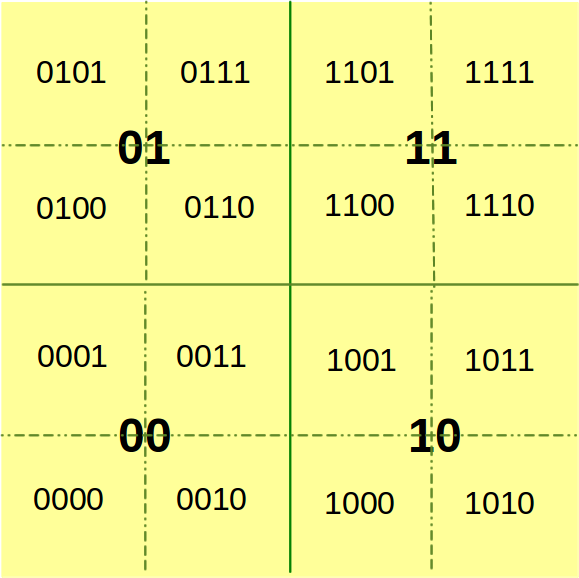
\includegraphics[width=0.25\textwidth]{MongoIndex}
\caption{Representation of geohash values for eight quadrants}
\label{figmongoindex}
\end{figure}
MongoDB also provide another 2d index optimized, called Haystack index, to return the results in small areas and is not supported by spherical query operations. To use haystack index in queries, \textit{\$geoSearch} command should be used. Actually, the ways which 2d and 2dsphere index could be applied, cannot access sometimes these small areas. MongoDB also uses B-Tree structure for other type of index, such as Single Field (e.g. indexing over names), Compound, and Text Index. 
%(Probably this point effect on the structure of geospatial index.)

MongoDB supports the following general operations to be executed with geospatial indexes through the mentioned operator:
\begin{itemize}
\item Inclusion: for locations contained entirely within a specified polygon which uses the \textit{\$geoWithin} function.
\item Intersection: for locations that cross or intersects with a geometry using the
\textit{\$geoIntersects} function.
\item Proximity: for locations that are near to a specified point by the \textit{\$near}
function. 
\end{itemize}
The way that the index structure should be applied varies in different queries. For instance, the geoNear command expects the collection to have at most only one 2d index and/or only one 2dsphere. The limitation have to be considered while using the operations or commands. 
%mongoformat

%http://www.bigfastblog.com/geohash-intro
%http://wiki.gis.com/wiki/index.php/Geohash
%wikipedia
%http://batchgeocode.net/what-is-geohash/
%http://blog.cobrain.com/2013/09/18/intro-to-geohashing/

\subsubsection{MarkLogic Server 7}
Geospatial data in MarkLogic is encoded as XML elements and/or attributes in different representations. MarkLogic handles the geospatial data in GML, KML, GeoRss, WKT and even a general format for geometric data which are not based on a specified format as explained in~\cite{marklogicGeo}. Similar to MongoDB, WGS84 and the raw coordinate systems are supported for geospatial data. WGS84 is used for data on Earth and the raw coordinate system is suitable for the data on the flat plane.

Regarding the geospatial queries, the following types are supported,
\begin{itemize}
\item Point query: Queries matching a single point.
\item Box query: Queries searching for any point within a rectangular box.
\item Radius query: Queries searching for any point within a specified distance around a point.
\item Polygon query: Queries finding any point within a specified n-sided polygon.
\end{itemize}
To do the geospatial queries, numerous geospatial query constructors exist as well as geospatial operators as built-in functions to perform the operations.
Here, some of these operators are listed,
\begin{itemize}
\item box-intersects: Returns true if the box intersects with the given region.
\item circle-intersects: Returns true if the circle intersects with the given region.
\item polygon-intersects: Returns true if the polygon intersects with the specified region.
\item complex-polygon-intersects: Returns true if the complex-polygon intersects with the given region. A complex polygon is a polygon which is not convex or concave.
\item polygon-contains: Returns true if the polygon contains the defined region.
\item complex-polygon-contains: Returns true if the complex-polygon contains the given region.
\item distance: Returns the distance (in miles) between two points.
\item shortest-distance: Returns the great circle distance between a point and an region. 
\item destination: Returns the point at the given distance along the given direction from the starting point.
\end{itemize}
The region in these operations is a circle, box, polygon, linestring, or complex-polygon 
which is defined by a \textit{region} constructor.
The geospatial query constructors build the queries on the geospatial data. 
Depending on the use case, the relevant constructors and functions from the correspondent namespace should be applied. For instance, if we want to query data expressed in both GML and KML, the \textit{geo} namespace functions are the best choice since they support the queries in all supported geospatial formats.
Also for data in geoRSS, the functions in \textit{georss} namespace could be used. 
This concept is shown in Code~\ref{marklogic-region} which searches for the points inside the specified region. 
\vspace{10px}
\begin{fakeXML}[escapechar=\%,label=marklogic-region,caption=A query example in MarkLogic]
...
xdmp:document-insert("/points.xml",
<root xmlns:geo="http://marklogic.com/geospatial">
  <item><gml:Point><gml:pos>10.5 30.0</gml:pos></gml:Point></item>
  <item><georss:point>15.35 35.34</georss:point></item>
  <item><Dot Latitude="5.11" Longitude="40.55"/></item>
</root> );
 ...
cts:search(doc("/points.xml")//item, 
 geo:geospatial-query(
   geo:box(
     <gml:Envelope>
       <gml:lowerCorner>10.0 35.0</gml:lowerCorner>
       <gml:upperCorner>20.0 40.0</gml:upperCorner>
     </gml:Envelope>)
 ))
 
 %\colorbox{light-gray}{Result}% : <item><georss:point>15.35 35.34</georss:point></item>
 \end{fakeXML}
\vspace{10px}
Another example represented in Code~\ref{marklogic-path} shows how MarkLogic returns the 
points in a given path which lie inside the defined region.
\vspace{10px}
\begin{fakeXML}[escapechar=\%,label=marklogic-path,caption=Another query example in MarkLogic]
cts:search(doc("/points.xml")//item,
  cts:path-geospatial-query("/root/item/point", 
  			cts:box(10.0, 35.0, 20.0, 40.0)))
\end{fakeXML}
\vspace{10px}

Primitive types are another fact in the geospatial queries which might be needed in query conditions 
as shown in the previous Codes~\ref{marklogic-region} and \ref{marklogic-path} using the \textit{box} constructor. These types as instancs of the base type \textit{region}, encompassing \textit{box}, \textit{circle}, \textit{complex-polygon}, \textit{linestring}, \textit{point}, and \textit{polygon}. For instance, the contents of the polygon element in the document "zip.xml" can be cast to a \textit{cts:polygon} using the \textit{cts:polygon} constructor as in the following,
\vspace{10px}
\begin{fakeJSON}
cts:polygon(fn:data(fn:doc("zip.xml")//polygon[@id eq "712"]))
\end{fakeJSON}
\vspace{10px}
%Latitudes and longitude pairs shape points. Points shape other geometries, such as circle or polygon. Boxes are formed by 4 points which on the surface of Earth. The edges of the box are arcs, but when those arcs are projected into a plane, they become two-dimensional latitude and longitude lines, and the space defined by those lines forms a rectangle. A linestring is a sequence of connected joined arcs that do not necessarily form a closed loop. 

Marklogic also provides functions to handle the WKT datatype. The function \textit{parse-wkt} reads WKT into the \textit{region} items as the following example returns a polygon.
\vspace{10px}
\begin{fakeJSON}
cts:parse-wkt("POINT(10 10)")
\end{fakeJSON}
\vspace{10px}
This point can be used in queries as any other type. Conversly the function \textit{to-wkt} converts \textit{region} type to WKT.


\textbf{The Geospatial Index.}
Geospatial index in MarkLogic is not based on neither the quad tree nor R-tree. It works similar to a range index with points as data values. In this range index, every value is a pair of latitude (lat) and longitude (long). Like an array of x,y values, sorted mainly based on latitude and then longitude values. The values in this array are also connected to the corresponding document.
The points would be founded easily in a sorted structure. 
Boxes could be found first by finding the latitude range, then checking for the longitude range. 
For circles and polygons as well as more complex types, the geometry's bounding box is used to find the region they belong to. 
Also, to check whether a point is inside the polygon, the number of intersections with the northward or southward arc of the point is counted.
\vspace{10px}
\begin{table}
\centering
\begin{tabular}{|l |l |}\hline
\textbf{Data} & \textbf{Path}\\\hline
\begin{fakeJSON}
<a:geo>
  <a:location>37 -122</a:location>
</a:geo>
\end{fakeJSON} &
\begin{fakeJSON}
/a:geo/a:location
\end{fakeJSON}\\\hline
\begin{fakeJSON}
<a:geo>
  <a:location data:"37 -122/>
</a:geo>
\end{fakeJSON} &
\begin{fakeJSON}
/a:geo/a:location/@data
\end{fakeJSON}
\\\hline
\end{tabular}
\caption{Data and the related path for indexing in MarkLogic}
\label{t.pathindexmarklogic}
\end{table}
\vspace{10px}
Based on this structure, Marklogic supports the following geospatial indexes,
\begin{itemize}
\item Geospatial Element Indexes: With this index, the data is represented by whitespace or punctuation separated element content. The lat-long or long-lat point formats could represent a point. Other entries such as z-coordinate or altitudes will be omitted.
\item Geospatial Element Child Indexes: With this index, the data comes only from the elements that are a specific child of a specific element containing whitespace or punctuation separated content.
\item Geospatial Element Pair Indexes: In this index, the data is considered from specific pair of elements that are a child of another specific element.
\item Geospatial Attribute Pair Indexes: With this index, the data is involved in a pair of specific attributes of a particular element.
\item Geospatial Path Range Indexes: With this index, the data is expressed in the same manner as a geospatial element index and the element or attribute index is defined by a path expression. Table~\ref{t.pathindexmarklogic} shows two examples of the data as an element and attribute and related paths for indexing each one. It should be mentioned that a defined path cannot be replaced with a new one unless it is removed.
\end{itemize}

To speed up the retrieval of geospatial values geospatial indexes enable geospatial lexicon lookups. Since these functions are implemented using geospatial indexes, the appropriate index must be created in order to use a geospatial lexicon. As an example, a geospatial element index is needed to use the \textit{element-geospatial-boxes}. Here is a sample to show how these functions are used and returns values from the specified element geospatial value lexicon that match the specified wildcard pattern.
\vspace{10px}
\begin{fakeJSON}[escapechar=\!]
cts:element-geospatial-value-match(xs:QName("point"),
cts:point(10,20))

!\colorbox{light-gray}{Result}! : 10,20
\end{fakeJSON}
\vspace{10px}

For querying on geospatial data in MarkLogic, after loading the data into the database and making the indexes, primitive types should be constructed to be used in query functions. Then, geospatial queries are constructed using these primitive types. 

\subsubsection{eXist-db}
%Here, we briefly describe the concepts of geospatial support in eXist-db\footnote{The spatial module in eXist-db is still in experimental satus.} to see the properties and implementation model of the functions and the index structure. 

eXist-db~\cite{existdb} version $1.2$\footnote{The spatial module in eXist-db is still in experimental status.} supports geospatial data in GML $2.1.2$ format. The geospatial features are provided using the JTS API in geospatial computations. 
The general development idea of indexing in eXist-db follows a modular architecture.
The geospatial index is developed based on this model and maintained as a pluggable extension. 
%To create the geospatial index, it must be configured in collection-specific configuration XML files that are located in the system collection: "/db/system/config". 
eXist-db connects to a relational database to index spatial data. The index doesn't store character data from the document. Instead, WKB index entries are stored through the JDBC in the HSQLDB or any other relational database namely PostGIS. 

The index creation relies on the open source libraries of the GeoTools~\cite{geotools} project. Geometries are stored both in the original coordinate system and WGS84 system in index structure to allow the operations on data originated from the different systems. In this way, transformations between coordinate systems are included using GeoTools library.
 
%In other words, the spatial data is stored in the DB, but geometries, as JTS Geometry instances, are held in memory, waiting for a special mode to be flushed into a relational DB, insertion or removal. The Geometry WKT representation would be serialized and deserialized to and from the database.

To query a spatial dataset, the spatial index and the spatial module must be enabled in the main configuration file (conf.xml). The following content in a configuration file of a collection in a database configures the spatial index on GML geometries. 
\vspace{10px}
\begin{fakeJSON}
<collection xmlns="http://exist-db.org/collection-config/1.0">
  <index>
    <gml flushAfter="200"/>
  </index>
</collection>
\end{fakeJSON}
\vspace{10px}
The attribute \textit{flushAfter="200"} says that the index entries in memory will be flushed into the HSQLDB. Now, the dataset is ready to query and Code~\ref{} is a sample query that return the whole polygons which intersect with the second argument of the \textit{spatial:intersects} function.
\begin{fakeXML}[label=intersectexist,caption=A spatial sample query in eXist-db using \textit{spatial:intersects} function]
declare namespace gml = "http://www.opengis.net/gml";
spatial:intersects(//gml:Polygon,
  <gml:Polygon srsName="osgb:BNG" xmlns:gml='http://www.opengis.net/gml'>
    <gml:outerBoundaryIs>
      <gml:LinearRing>
        <gml:coordinates>
	  08.278200,187600 278400,187600 278400,188000 278200,188000 278200,187600
	</gml:coordinates>
      </gml:LinearRing>
    </gml:outerBoundaryIs>
  </gml:Polygon>
) 
\end{fakeXML}
\subsubsection{MonetDB}
MonetDB\footnote{This information which are presented here, are from January 2014 Bugfix.} basically is a relational column-store database which has implemented a separate module to support the objects and functions in the OGC "Simple Features Specification for SQL"~\cite{ogcsfs}. The current implementation of spatial support is still simple. MonetDB stores XML in its relational architecture as Boncz et al~\cite{Boncz2006} describes. The geospatial component in MonetDB wraps the open source GEOS libraries~\cite{GEOS}
which is the \textit{C++} implementation of the JTS API. When \textit{geom}, the geospatial module in MonetDB/SQL component, is enabled, then the created databases are spatially-enabled by default. MonetDB supports the OGC geospatial types. Besides, a non-OGC type, called \textit{mbr}, is used for stroing a 2D box for fast access. Numerous functions exist in MonetDB to provide SQL-based geospatial querying. These functions are categorized in geometry constructors, functions an specific geometry, and functions on bounding boxes. Function on boxes could be used for pre-filtering in some complicated queries. Below shows some geospatial functions that can be used in queries.
\begin{itemize}
\item \textbf{\texttt{ST\char`_GeometryFromText(wkt string)}}, which creates a geometry out of WKT string.
\item \textbf{\texttt{ST\char`_AsText(geom Geometry)}}, which returns the WKT representation of the Geometry.
\item \textbf{\texttt{ST\char`_ConvexHull(geom Geometry)}}, which returns the convex hull of the Geometry in the Geometry format.
\item \textbf{\texttt{ST\char`_InteriorRingN(geom Polygon, ringNum integer)}}, which returns the n-th interior ring of the Polygon as a linestring.
\item \textbf{\texttt{ST\char`_IsRing(geom LineString)}}, which returns a boolean value showing whether the LineString is both closed and simple or not.
\item \textbf{\texttt{ST\char`_XMax(box mbr)}/\texttt{ST\char`_XMax(geom Geometry)}}, which returns the maximum $X$ coordintate of the provided bounding box. In latter case which a 2D geometry is provided, first its bounding box is computed.
\item \textbf{mbr(geom Geometry)}, which returns the minimum bounding box created for the geometry.
\item \textbf{@} (mbrContained function), which returns a boolean value expressing whether box1 is contained by box2 in \textit{box1:mbr @ box2:mbr}.
\item \textbf{\&\&} (mbrOverlaps function), which returns a boolean value showing whether two bounding boxes overlap in \textit{box1:mbr \&\& box2:mbr}.

\end{itemize}

The following example returns a geometry form \\textit{spatial} table:
\vspace{10px}
\begin{fakeJSON}[escapechar=\!]
!\textbf{SELECT}! PointFromText('POINT(' || long || ' ' || lat || ')') !\textbf{FROM}! spatial !\textbf{LIMIT}! 1;
\end{fakeJSON}
\vspace{10px}

As Vermeij et al~\cite{MonetDB} discusses, MonetDB benefits from the design principles for spatial query processing in three main areas. First, the column-based storage approach keeps the non-needed geometry out of the way since the traditional tuple-based storage model stores the whole tuple physically together on a disk block. Additionally, some efficient filtering stored in the same column and some approximate geometries, e.g. minimum bounding box, maximum enclosed circle, and maximum enclosed rectangle stored in other related tables would speed up the queries as the index structure does. Second, MonetDB query optimizer effectively improves the geospatial query performance. Third, the spatial data types integration with XML types in MonetDB is considered as an efficient way of querying. 
%Even though MonetDB still does not provide any indexing structure, ....
%\begin{itemize}
%\item The column-store approach of MonetDB is advantagous for geospatial data, since skips the unnecessary %attributes. This becomes important as only a fraction of data is needed in most of 
%\end{itemize}


\subsection{Other Related Topics}

In addition to the aforementioned topics, some other areas have been discovered as well in this research line. 
we briefly discuss here two ideas which might be advantageous 
for more geospatial features and processing in a geospatial database.
The first idea, presented in the first paragraph, is about the unification of the coordinate system when the data
is coming from different sources. The second idea, presented in the second paragraph, is pointing to a 
completely different idea of finding a path between to points in these database.

Schwarz et al~\cite{Schwarz2004} introduced a library for geospatial data management to enable handling the different coordinate systems. This library provides geospatial functions which are delegated to JTS library. As mentioned before, JTS library only supports the Cartesian coordinate system and the input geometries should be in a common systems to be processed. It can happen that the geometries have different coordinate systems. For example, the geospatial data is provided from different sources. In order to work with JTS library, a common coordinate system is chosen to which other systems of the current data is converted. This coordinate system is chosen considering the the transformation issues to have the minimum differences from the original data and to maximize the transformations precision.


Padmaja et al~\cite{short-path} introduces an alternative way of finding the shortest path regarding existing cost. The k-shortest path and many other path finding algorithms are efficient as long as the effecting cost factors do not change dynamically. This provided method first finds the shortest paths without considering the cost factors. At the end, the factors are used to rank the paths. All paths between each two points could be stored in database in pre-processing stage to reduce the further combinations. To find the paths, each edge in the network of the connected points should be provided with the start and end points. The process starts from the starting point and finds the whole connected ones and continues till reaches the destination. The paths would be obtained by joining the edges detected in each step.
















\newpage
\section{Spatial Querying in BaseX}
\label{s.basex}
%TODO tozihe bishtar dar more requirements va inke chera injuri develop shode
%TODO:why gml:http://www.w3.org/Mobile/posdep/GMLIntroduction.html - 
%TODO: and  http://spatialnews.geocomm.com/features/gml/topten.html
Spatial query is a special type of query which requires the processing of geometries with two certain properties in general. First, it has geometries as inputs and outputs as well as other primitive types, like double, integer, etc. Second, it considers spatial relations between the geometries.
As we discussed in Section~\ref{s.dbs}, there are various viewpoints in providing geospatial features in a database to fulfill the expected requirements. Following the OGC Simple Feature (OGCSF)~\cite{springergeo} data model, geospatial features in BaseX adapt the specification of EXPath geospatial API function interface. This specification defines commonly used functions from the OGCSF Common Access API~\cite{simpleFeature}. Since the OGCSF data model is typically represented in GML, we concentrate to add the support of GML format in BaseX. However, an implementation could support other encodings such as KML. 

Throughout the following sections, we discuss the integration of geospatial data processing in BaseX. We introduce geospatial functions as a new module, called \textit{Geo Module}, in Section~\ref{geomodule}. Query efficiency is improved later in Section~\ref{indexBX} by implementing an index structure. Indexing and the related time complexities are discussed hereafter in Section~\ref{indexFunc} and Section~\ref{BXevaluation}, as the critical issue in this topic. Finally, the concluding points are explained in Section~\ref{BXconc}.

\subsection{Geo Module}
\label{geomodule}
As mentioned above, geospatial features in BaseX are implemented based on the EXPath Geo Module Specification~\cite{expath}. This specification contains the definition of functions for widely used geographic and geometric analysis operations, from OGCSF Common Access API version $1.2$. These functions apply to geometries in different formats, such as GML, KML, GeoJSON, Well Known Text (WKT), and even Well Known Binary (WKB). Based on the specification, Geo Module in BaseX comprises a set of functions, like intersection, within, distance, boundary, centroid, diference, and union, added to the \textit{basex-api} package. The geometries supported in this module are Point, LineString, Polygon, MultiPoint, MultiLineString, and MultiPolygon. This module is an individual package with a set of classes as briefly described below,
\begin{itemize}
\item \textit{Geo}: This class is the main class, in which all geospatial functions are defined. The set of functions in this class is provided to be directly used in XQuery statements. The complete list of functions and their description are available in the online BaseX documentation~\cite{basexgeo}.
\item \textit{GeoError}: This class defines error functions with related massages which are thrown when an error occurs.
\item \textit{GeoTest}: Test functions for the \textit{Geo} class are implemented here.
\item \textit{GmlReader}: Functions required to parse GML geometries as XML elements are implemented in this class.
\item \textit{GeoIndex}: This class implements the functions related to the geospatial index. 
\end{itemize}

Geospatial index structure is implemented in BaseX core. Spatial indexing and related implementation details will be described in Section~\ref{indexBX}. Here, we explain general functionalities of this module.

The geospatial functions are defined as public methods in the \textit{Geo} class. They use some private methods to read geometries or write them out into the GUI. Besides, each function employs the corresponding function from the JTS library to do the required geometric operation and provide the appropriate result. Here, we shortly explain how the input geometries, either from a variable or a database node, are processed.


Suppose we are searching for all geometries within the specified polygon $\$p$. The query should be written using XQuery via BaseX GUI as follows,
\vspace{10px}
\begin{fakeJSON}
let $p := 
<gml:Polygon>
  <gml:outerBoundaryIs> ... </gml:outerBoundaryIs>
</gml:Polygon>
for $x in //gml:Polygon
  return if ( within($x, $p) ) then $x else ()
\end{fakeJSON}
\vspace{10px}
Each geospatial function has at least one geometry as input, as in the above function \textit{within}. In this example, the variable $\$p$ is provided as a document node and the variable $\$x$ iterates all Polygon nodes in the current database. Various functions are involved in processing this query. Followings, this process which is illustrated in Figure~\ref{figGeoModuleProcess} is explained in detail. 

To read the geometries as a document node, the private function \textit{geo} makes sure that the node name is at least a valid geometry name. It means that if the element name is not contained in the set of geometry names, this function will throw an error. 
Then, the GmlReader class is used to read and parse the whole element and to check the validity based on GML $2.0$ format. Regarding the JTS limitation, geometries have to be in GML $2.0$ format to be validated and analyzed for further operations. 

The aforementioned GmlReader class reads the elements differently based on their types, i.e., tag names. If the element is a valid GML geometry, the function creates the corresponding geometry, using JTS constructors. Otherwise, the matching error massage will be shown. For instance, if a polygon does not have any outer ring or if the coordinates of a ring do not shape a closed ring, an error will be thrown. 

 \begin{figure}
\centering
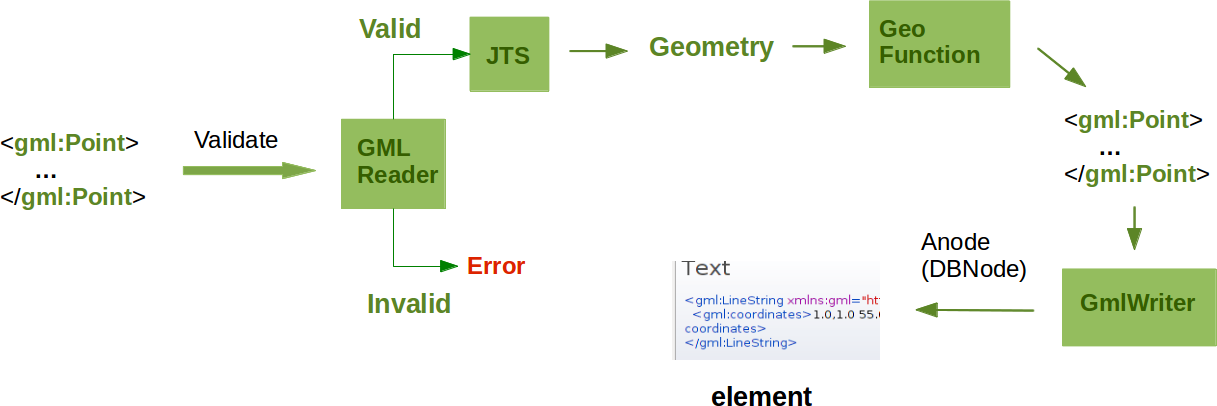
\includegraphics[width=0.95\textwidth]{GeoModuleProcess}
\caption{Converting GML elements to geometries}
\label{figGeoModuleProcess}
\end{figure}

Now, the geometries are ready to be processed in geometric operations, like:
\begin{itemize}
\item checking two geometries whether they intersect each other
\item finding the symmetric distance of two geometries
\item getting the number of inner rings of a polygon.
\end{itemize}
These operations are done using the JTS functions. The output could be either in any XML Schema (XSD) data types such as integer, boolean, string, and URI or GML Geometry. The XSD type are equivalent to the BaseX defined data types. For example, the primitve data types boolean, integer, and string are represented in BaseX as the classes \textit{Bln}, \textit{Str}, and \textit{Int}, respectively. In addition, the Geometry type which is the output of functions like intersection, union, and difference of two geometries, must be returned as an element in the abstract node type (\textit{ANode}) to be in compliance with the specification. Having the output geometries in GML format, GMLWriter function converts them first to a string, using JTS GmlWriter and builds a database node (\textit{DBNode}) hereafter. Considering the point that DBNode extends ANode, the output node is sent to the GUI and is shown as a GML element, expressing the geometric result. 

Now, it time to discuss the query performance that seems not satisfying. Having commonly huge geospatial data, we encounter serious performance problems. The common solution is an indexing algorithm designed to improve efficiency. Since the geospatial data is a written form of geometries positioned in the space, an indexing structure should be designed considering the positions. In the following sections, we discuss an indexing approach and its influence on performance compared with the querying without using any geospatial index.


\subsection{Geospatial Index in BaseX}
\label{indexBX}
To enhance the geospatial query time in BaseX, we discuss an index structure. This index avoids processing the whole database when partial checking of the file would be enough. For this purpose, a bounding box is computed for each geometry by which an efficient filtering can be applied. For example, if we want to find the objects within a specific geometry, examining just the area near to this geometry is adequate. If two geometries have intersecting bounding boxes, they might intersect each other and have to be checked wether they fulfill the query condition. Otherwise, they will not have any contact and there is no need to check them. This approach decreases the number of scanned geometries and consequently gives the better timing, which we call it two step filtering. The two step filtering is clarified as followings,
\begin{enumerate}
\item Finding the geometries which their bounding box intersect with the bounding box of query area
\item Checking the selected geometries against the query condition
\end{enumerate}
%Moreover, functions of this module in which a big number of geometries from the database coule be involved, have the time complexity bigger than O(1) and need a spatial indexing to be handled in shorter time. %TODO conintinue


 \begin{figure}
\centering
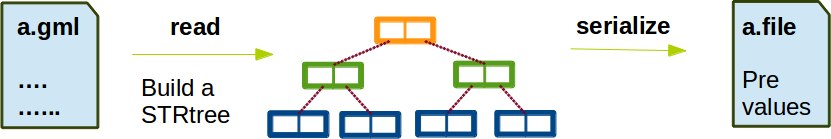
\includegraphics[width=0.95\textwidth]{IndexinFile}
\caption{Geospatial index creation}
\label{figIndexinFile}
\end{figure}

Among the spatial index structures discussed in Section~\ref{s.geospatial-index}, JTS supports the STR-tree and Quad-tree. Davis~\cite{jts-presentation} discussed that STR-tree in contrast with Quad-tree can not be updated after the generation. However, we choose the STR-tree since it has better performance for our performance as we discussed in Section~\ref{indexsummary}. As mentioned before, STR-tree has the basic of R-Tree with the improved performance. The index tree, holding the bounding boxes in inner nodes and geometries in leaves, is made once when the spatial index for the database is requested. Then, this structure is stored in a file on disk. This process is illustrated in Figure~\ref{figIndexinFile}. Each time the index is requested, the file is read 
into main memory and will be kept there for future requests.
At the end, the two step filltering is executed. 
It should be mentioned that only the following queries would benefit from this index. The definitions of these functions are provided in EXPath Geo Module specification.
\begin{itemize}
\item intersects (geometry1, geometry2)
\item within (geometry1, geometry2)
\item contains (geometry1, geometry2)
\item overlaps (geometry1, geometry2)
\item crosses (geometry1, geometry2)
\item touches (geometry1, geometry2)
\end{itemize}

The geospatial index structure is involved both in BaseX core and the \textit{basex-api} package. The main structure of index is added as a package in core, called \textit{index.spatial}. This package contains the index builder classes based on the core index structure of BaseX. The class \textit{SpatialBuilder} which extends \textit{IndexBuilder}, builds the index tree using pre-values instead of the tag names to address the database elements. Then, the JTS serializer writes this tree into a file, called \textit{STR-treeIndex}.

The other \textit{GeoIndex} class in the \textit{basex-api} package extends \textit{QueryModule} and implements the method defined by the JTS STR-tree class for reading the index file from hard disk into memory. Additionally, this class implements the \textit{filter} method to do the first step of two step filtering. The datails of the index implementation is described in the following section.
 
\subsection{Index Functions Implementation}
\label{indexFunc}
To add the geospatial index, we tought of two approaches. The first approach implements new signature for the aforementioned functions in a new class. It means that the index filter function is encoded directly in the existing geo functions. Then, queries can be done with the new spatial function as in Code~\ref{intersectIndx}. In this query, the function \textit{geo-index:intersects} in the new namespace and signature applies the index functionalities inside the function. Therefore, we have two \textit{intersects} functions.
\vspace{10px}
\begin{fakeXML}[label=intersectIndx,caption=The geo function containing the index functions]
import module namespace geo-index = "http://expath.org/ns/GeoIndex";
let $a:= <gml:Polygon> ... </gml:Polygon>
return geo-index:intersects("DB", $a) 
\end{fakeXML}

\vspace{10px}
\begin{fakeXML}[label=geoandfilter,caption=Geo function used with index function]
import module namespace geo-index = "http://expath.org/ns/GeoIndex";
import module namespace geo = "http://expath.org/ns/Geo";
declare namespace gml="http://www.opengis.net/gml";
let $a:= <gml:Polygon>
                <gml:outerBoundaryIs>
                  <gml:LinearRing>
              	    <gml:coordinates>
              	      3.9,50.6 6,52.8 4.5,52.8 3.9,50.6
              	    </gml:coordinates>
                  </gml:LinearRing>
                </gml:outerBoundaryIs>
             </gml:Polygon>
return ( geo-index:filter("DB", $a)[geo:intersects( $a, .)])
\end{fakeXML}
\vspace{10px}

Since having two functions with the same name and functionality is redundant, we introduce a new approach in which the \textit{filter} function can be used in XQuery to benefit from the index structure. A sample query of this approach in Code~\ref{geoandfilter}, filters the geometries by the \textit{geo-index:filter} function. Next, the \textit{geo:intersects} function of Geo Module is applied to the filtered geometries. To summarize, the former approach does the whole process including the first step of filtering through the \textit{geo-index:intersects} function, while the latter uses the original \textit{geo:intersects} function together with \textit{geo-index:filter} which does the first step of filtering. 


The negative point about the second approach is that the input polygon, like polygon $\$a$ in Code~\ref{geoandfilter}, is read, parsed, and created every time that the spatial function, here \textit{intersects}, is called in the \textit{for} loop, even though it is the same fixed object. Since, this causes redundancy and consumes a considerable amount of time, we use a map to hash the fixed input and prevent the further redundant readings. This will dramatically reduce the query time, as shown in Figure~\ref{figMap}.
 \begin{figure}
\centering
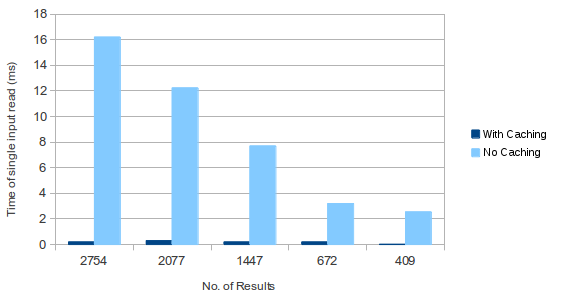
\includegraphics[width=0.9\textwidth]{MapIndexing}
\caption{Using a Map to cache the input geometry: performance effect}
\label{figMap}
\end{figure}

Figure~\ref{figMap} demonstrates the time consumed by different queries to read the single input geometry with or without caching. It could be seen that when no map is used, as the number of results goes higher more time is taken. In contrast, by caching the single input reading time remains constant, since the input geometry is read once. In other words, without caching the input geometry will be read each time the function \textit{geo:intersects} is called, as it is one of the input arguments. In the next section, we assess the performance issues related to the geospatial index.

\subsection{Evaluation and Improvement}
\label{BXevaluation}
%TODO:jomle aval beravad b sectione ghabl
There is no need to emphasize on the importance of role that indexing plays in the query time and performance improvement. Here, we use real-world data to observe the effect of currently implemented geospatial index, followed by in depth looking at the implementation from other perspectives. The aim is to find ways in order to improve performance. This data is provided by University of Twente, Department of Geoinformation Processing and holds some real information on Earth in GML $2.0$ format. The original file is based on one of the Netherlands coordinate system (RD/NAP Amersfoort RD New) and is around $133.3$ MB including $12773$ polygons inside $11886$ multipolygons.
We run different queries on this data with and without geospatial index to see time consumption dependency on the index structure. 
\begin{figure}
\centering
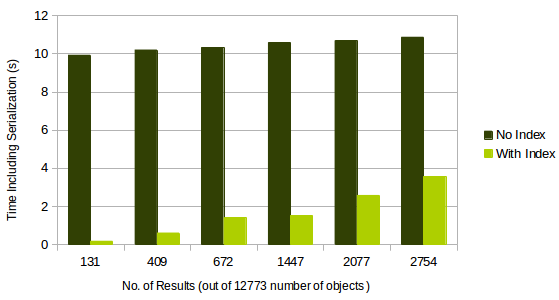
\includegraphics[width=0.85\textwidth]{IndexEfficiency-2}
\caption{Query performance improvement by using geospatial index}
\label{figIndexEfficiency}
\end{figure}

Since queries have various number of results, we can see the trend changes in regards to the number of outputs.
To start with, we take a look at the effect on index utilization in queries in comparison with queries using no geospatial index. Figure~\ref{figIndexEfficiency} represents the effectiveness of index utilization.
As shown in Figure~\ref{figIndexEfficiency}, when geospatial index is not used, the query time remains constant for every query regardless of the number of results. As we discussed in Section~\ref{indexBX}, this is due to the fact that the whole file is scanned and analyzed for each query. In contrast, queries using geospatial index relatively take more time as the number of output objects goes higher. It confirms that the filtering approach is going in the right direction, but the performance still is not satisfying. Thus, we need to investigate more to improve it.
\begin{figure}
\centering
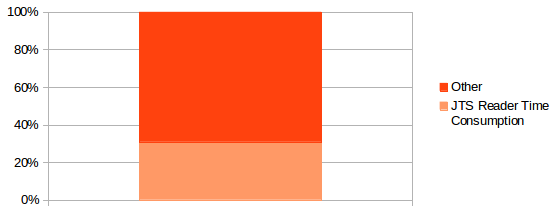
\includegraphics[width=0.8\textwidth]{JTSReadetTimeConsumption}
\caption{JTSReader time consumpion in total query time}
\label{figJTSReaderTime}
\end{figure}

By monitoring the times consumed by different parts of a query, we discovered that JTS GMLReader functions take considerable amount of time according to the Figure~\ref{figJTSReaderTime}. This figure depicts that the Reader consumes nearly $30\%$ of the whole query time. JTS GMLReader operates this part that reads the geometries from GML and converts them to JTS geometries. 
\begin{figure}
\centering
\subfigure[Through JTS GMLReader]{
	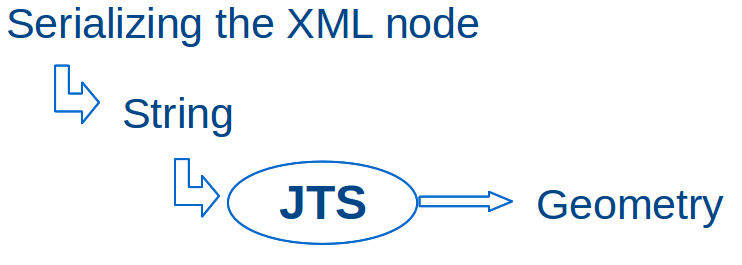
\includegraphics[width=0.47\textwidth]{GmlReaderProcess1.png}
	\label{figParseProcess1}
}
\centering
\subfigure[Through Custom GML Reader]{
	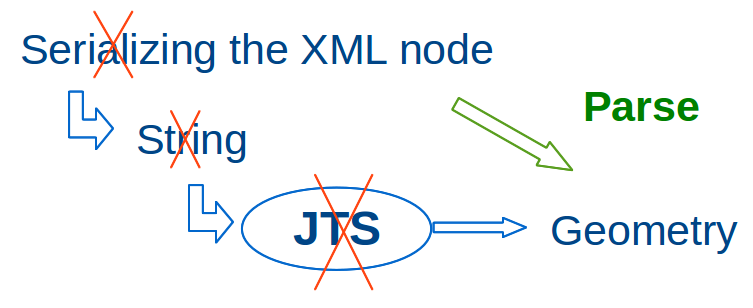
\includegraphics[width=0.47\textwidth]{GmlReaderProcess.png}
	\label{figParseProcess2}
	
}
\caption{Parsing process of the GML elements}
\label{figParseProcess}
\end{figure}
Regarding the geometry reading process by JTS, shown in Figure~\ref{figParseProcess1}, it seems that the three steps serializing the XML, converting it to string, and constructing geometries by JTS can be eliminated and directly parsing approach might decline the query time. Thus, we implement a costume GML reader class to immediately parse the GML elements into the JTS geometries (see Figure~\ref{figParseProcess2}). To assess the time efficiency, a set of queries are tested and the results are presented in Figure~\ref{figGmlReader}. 
\begin{figure}
\centering
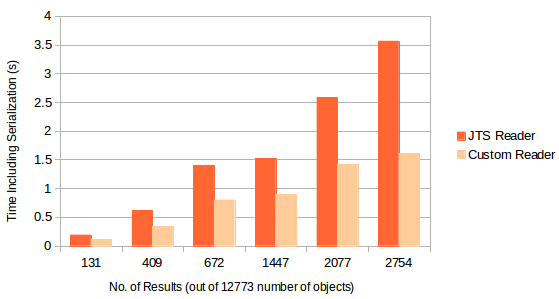
\includegraphics[width=0.8\textwidth]{GmlReader-2}
\caption{Custom GMLReader vs. JTS GMLReaer}
\label{figGmlReader}
\end{figure}
As it was supposed, reading time drastically reduced by use of the new reader functions, although both have increasing trend proportional to the number of outputs.%gosaste

A deeper look at the different parts of a query will be beneficial to find the parts where need to be improved. Suppose we run the query below,
\vspace{10px}
\begin{fakeJSON}
let $a:= <gml:Polygon> ... </gml:Polygon>
return ( geo-index:filter("DB", $a) [geo:intersects( . , $a)]).
\end{fakeJSON}
\vspace{10px}
The total query time will be divided into the following parts,

\begin{enumerate}
\item reading the input geometry $\$a$
\item filtering the geometries using \textit{filter} function by pre values 
\item reading the filtered geometries from the database using selected pre values
\item apply \textit{intersects} operation on the pair of input geometry and each selected geometry.
\end{enumerate}

To see how each part influence the performance, we examine them separately. Figure~\ref{figDetailedTiming} shows the times taken by the above-mentioned actions. It could be seen that the biggest amount of time is spent reading the geometries. Even reading the single input geometry seems to be expensive. Hence, the reading function should be observed more in detail.

\begin{figure}
\centering
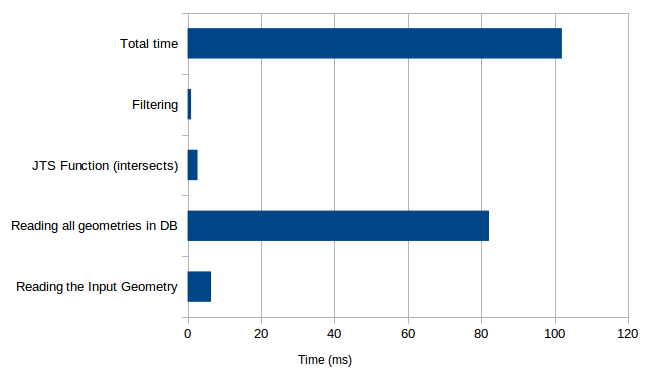
\includegraphics[width=0.7\textwidth,height=0.2\textheight]{detailedTiming}
\caption{Detailed timing in a query using geospatial index}
\label{figDetailedTiming}
\end{figure}


We have used the Java profiling to get more precise information. The first few methods in profile output with the highest percentage of time occupation, ordered from the most-used to the least-used, are listed in Table~\ref{javaprofile}.
\begin{table}
\begin{tabular}{l l l c l}
\textbf{rank} & \textbf{self} & \textbf{accum} & \textbf{count} & \textbf{method} \\
 & & & &\\
1 & 6.95\% & 6.95\% & 94 & org.basex.util.Token.{\color{red}split}\\
2 & 5.33\% & 12.28\% & 72 & org.expath.ns.GmlReader.createPolygon \\
3 & 4.59\% & 16.86\% & 62 & org.basex.util.Token.{\color{red}split} \\
4 & 4.22\% & 21.08\% & 57 & org.basex.query.func.JavaModuleFunc.eval \\
5 & 3.55\% & 24.63\% & 48 & org.expath.ns.Geo.geo \\
6 & 3.18\% & 27.81\% & 43 & org.basex.util.Token.{\color{red}split} \\
7 & 3.03\% & 30.84\% & 41 & org.basex.util.Token.{\color{red}split} \\
8 & 2.96\% & 33.80\% & 40 & org.basex.util.Token.{\color{red}split} \\
9 & 2.74\% & 36.54\% & 37 & org.expath.ns.Geo.geo \\
\end{tabular}
\caption{Java profiling output for the BaseX Geo Module}
\label{javaprofile}
\end{table}
As the profile output in Table~\ref{javaprofile} indicates, the \textit{split} function calls consume the greatest amount of time. Besides, \textit{createPolygon} and \textit{geo} functions used in \textit{GmlReader} class are expensive. Therefore, these functions should be focused in performance tuning. 
\begin{figure}
\centering
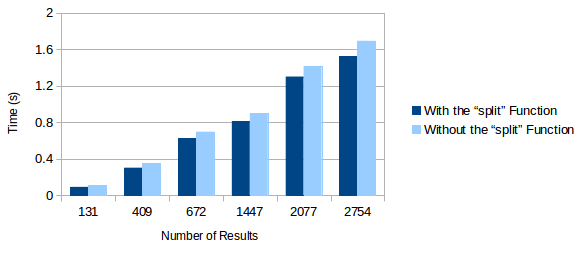
\includegraphics[width=0.8\textwidth,height=0.2\textheight]{BXSplit}
\caption{The query times of the selected queries before and after the removing of \textit{split} function}
\label{figBXSplit}
\end{figure}
Since the \textit{split} function has the most frequent call, we discard it in favour of better performance. This function is used to divide the string value of \textit{coordinate} tag regarding the delimiters to make coordinate pairs. We replaced it with a piece of code to parse this string. 
A coordinate value in GML $2.0$ can include different points which are separated with a space. Each point in a coordinate has two dimensions $X$ and $Y$ separated with a comma. Code~\ref{coord-example} shows an example of the GML $2.0$ coordinate. Based on this format, the new code reads the coordinate string and acts based on the position and type of delimiters and numbers. Therefore, the coordinate pairs are constructed from a valid string. Otherwise, an error massage will be shown. Figure~\ref{figBXSplit} shows the effect of removing the \textit{split} function on the query times. This Figure indicates that this effect grows as the number of results gets bigger.
 
\vspace{10px}
\begin{fakeXML}[label=coord-example,caption=An example of GML 2.0 coordinate]
<gml:coordinates>
  3.9,50.6 6,52.8 4.5,52.8 3.9,50.6
</gml:coordinates>
\end{fakeXML}
\vspace{10px}

In addition to the \textit{split} function, we omit the $Z$ values in parsing process, since the $Z$ value is ignored with the geospatial functions. It means that it is useless to read this value. It can be considered as a limitation of GML $2.0$ which is improved in GML $3.0$. Not surprisingly, excluding the $Z$ values from the parsing process declines the query time that is displayed in Figure~\ref{figBXZvalue}. This effect is minor in the smaller number of results and is more obvious with more output numbers.

\begin{figure}
\centering
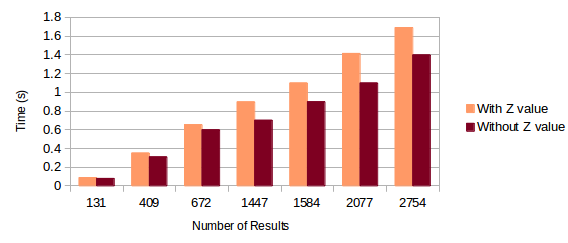
\includegraphics[width=0.8\textwidth,height=0.2\textheight]{BXZvalue-sec}
\caption{The effect of ignoring the $Z$ values of coordinates in GML parsing on query times}
\label{figBXZvalue}
\end{figure}

Up to this point we have tried various ways to decrease the query times in the Geo Module. Further attempts could be done following the aforementioned Java profiling list (Table~\ref{javaprofile}), if the implementation will be continued in the current direction.

\subsection{Conclusion}
\label{BXconc}
In this Section, we discussed the Geo Module implementation details and assessment in BaseX which provides a set of geometric functions based on the EXPath Geo Module specification. This module employs the JTS library to compute the geometric operations. To enhance the performance, the JTS STR-tree index structure is added that accelerates the execution time of queries such as intersects, within, inside, and touches. This is done by applying a filtering in the STR-tree structure and consequently reducing the number of processes in the database. Besides the index tree, a GML Reader class is developed to parse the gml elements directly regarding the inefficiency in JTS GMLReader. Although the timing results are convincing, there is room for improvements. For example, the functions \textit{split}, \textit{geo}, and \textit{createPolygon} can be modified in favour of better performance.

\newpage
\section{BaseX and MongoDB}
\label{s.mongo}
%TODO:Complete

An introduction of MongoDB geospatial features is provided before in Section~\ref{mongo}. In this section, we will have a more-detailed overview of these functionalities and a comparison between BaseX and MongoDB. However these two systems follow distinct approaches, it would be beneficial to review MongoDB as a rather new, recently developed, and widely used database system. MongoDB is among the few NOSQL systems providing geospatial features. Here, we will mainly see differences between these systems, particularly in performance of the same features. This comparison empowers us to improve the geospatial querying performance in BaseX. 

As we discussed in Section~\ref{mongo}, geospatial data can be represented in MongoDB either as planar or spherical maps. Since Earth is a spherical globe, the geospatial calculations on planar maps are only an approximation~\cite{coordsys,coordsys-mongo}. As an example, the measurement of distances in planar maps are accurate only in a small region. It means that the spherical maps are the better representation when the calculations are expected as real ones on Earth. As our goal is to assess some geospatial features of MongoDB and compare it with Basex Geo Module, we focus merely on the spherical approach. Correspondingly, WGS84 is used instead of legacy coordinate pairs to express the spherical maps. 

\vspace{10px}
\begin{fakeXML}[label=feature-collection,caption=A GeoJSON file containing a \textit{FeatureCollection} object]
{
  "type": "FeatureCollection",
  "features": [
    {
      "type": "Feature",
      "geometry": {
        "type": "Point",
        "coordinates": [102.0, 0.5]
      },
      "properties": {
        "prop0": "value0"
      }
    },
    {
      "type": "Feature",
      "geometry": {
        "type": "LineString",
        "coordinates": [
          [102.0, 0.0], [103.0, 1.0], [104.0, 0.0], [105.0, 1.0]
        ]
      },
      "properties": {
        "prop1": 0.0,
        "prop0": "value0"
      }
    }
  ]
}
\end{fakeXML}
\vspace{10px}


Geospatial operators of MongoDB for spherical data support the GeoJSON~\cite{www/geojson} format. GeoJSON is a human-readable encoding format for representing the geographical features using JSON standard. It consists of an object which describes a geometry, \textit{Feature}, or collection of \textit{Features}. The type of geometries must be one of these types: Point, LineString, Polygon, MultiPoint, MultiLineString, MultiPolygon, and GeometryCollection. A \textit{Feature} must have members with the names \textit{geometry} and \textit{properties}. A feature collection is an object with the type \textit{FeatureCollection} which must have a member with the name \textit{features}. Code~\ref{feature-collection} is an instance GeoJSON file with a \textit{FeatureCollection} object.

The version $2.4$ of MongoDB which we have used for our testings, supports only three geometry types Point, LineString, and Polygon\footnote{The version $2.6$ adds the support of MultiPoint, MultiLineString, MultiPolygon, GeometryCollection.}. As mentioned in Section~\ref{mongo}, a geospatial query in MongoDB can use \textit{geoIntersects}, \textit{geoWithin}, \textit{near}, and \textit{nearSphere} operators. In addition, there are geometry specifiers to define geometries in query conditions of these operators. For instance, the \textit{\$center} and \textit{\$centerSphere} are specifiers for a circle area in planar and spherical maps on which the user intends to do the query. Then, the user can find all geometries within a determined circular area. Another example is the \textit{\$maxDistance} specifier that determines the maximum distance from a point in order to find geometries within this particular distance. Geometry specifires are limited to, \textit{\$geometry}, \textit{\$maxDistance}, \textit{\$center}, \textit{\$centerSphere}, \textit{\$box}, and \textit{\$polygon}. An example demonstrating the usage of the specifiers in a query is,
\vspace{10px}
\begin{fakeJSON}
db.<collection>.find( { <location field> :
                         { $geoWithin :
                           { $centerSphere :
                              [ [ <x>, <y> ] , <radius> ] }
                      } } )
\end{fakeJSON}
 \vspace{10px}
 
In the following sections, we will discuss the query performance of these two databases. 
In Section~\ref{s.query}, we analyze specific test queries. Then, the assessment continues
utilizing the indexing structure in Section~\ref{index}. Later, the update functionality of databases is 
investigated in Section~\ref{update}. Finally, Section~\ref{conc} contains the conclusion and further work.

\subsection{Querying the Databases}
\label{s.query}
To analyze the database behaviour, designing the same test queries on the identical dataset is the most straight-forward approach. Based on the MongoDB geospatial features and properties, the Netherland test dataset must be changed. A brief explanation of the changes is provided here to clarify the rules and limitations. The main change was to either remove multipolygon from the dataset or transforming them to a set of distinct polygons, since multipolygon is not supported in the version of MongoDB that we have used. Besides, the coordinate system is converted to WGS84. At the end, there are $12773$ polygons and no multipolygons in the data file. Since the geometries are changed and the results would be different, we repeat all queries with the new dataset in BaseX.

To start with, the GeoJSON file containing the geometries is imported into MongoDB. This can be done  using Java API or Mongo Shell with appropriate \textit{mongoimport} command. There are limitations to consider while importing a GeoJSON file in MongoDB. The main one is the \textit{document} size limitation in a \textit{collection}. Document and collection are two concepts in MongoDB which correspond with a table and a record in this table, respectively. A collection can have one or more documents and a document is a set of key-values. A database contains one or more collections. To successfully import a document into a collection, it should be smaller than $16$MB. Since it is common to have large geometries in real-world geographic data files, this limitation can be a problem. Another limitation is that the $z$ coordinate is not supported in MongoDB. When a coordinate contains $z$ dimension, although those geometries are not processed, no error massage is shown during the import process and query. MultiPoint, MultiLineString, and MultiPolygon, which are not supported in MongoDB, are also skipped in queries without any error massage. 

The above-mentioned size limitation made us to change the file structure again.
When the file structure was in the form of Code~\ref{feature-collection}, 
an error message regarding the size limitation was thrown. 
When the GeoJSON file structure is changed to contain individual features as below,
this problem disappeared.
\vspace{10px}
\begin{fakeXML}[label=features,caption=A GeoJSON file restructured regarding the size limitation]
    {
      "type": "Feature",
      "geometry": {...},
      "properties": {...}
    },
    {
      "type": "Feature",
      "geometry": {...},
      "properties": {...}
    }, 
    { ... }, ..., { ... }
\end{fakeXML}
\vspace{10px}
%TODO:explain about the query difficulties and aggregation of the above structure
After importing the file, we examined the common features, i.e., intersection, within, 
functionalities in both databases.
%and near  
The queries in Code~\ref{basex-query} and Code~\ref{mongo-query} find the intersecting geometries from the Netherlands' dataset with the given polygon in BaseX and MongoDB, respectively. The polygon coordinates are determined for different queries in the following way. At first, the maximum and minimum coordinates are found in the dataset. After that, we generate different input polygons in regard to these boundaries. The polygons coordinate are altered such that the number of results differes in each query.
\vspace{10px}
\begin{fakeXML}[label=basex-query,caption=Example query of \textit{intersects} function in BaseX]
import module namespace geo = "http://expath.org/ns/Geo";
declare namespace gml="http://www.opengis.net/gml";
let $a:= <gml:Polygon>
              <gml:outerBoundaryIs>
                <gml:LinearRing>
                  <gml:coordinates>
                    6,52.6 6.1,52.6 6.1,53 6,53 6,52.6
                  </gml:coordinates>
                </gml:LinearRing>
              </gml:outerBoundaryIs>
            </gml:Polygon>
for $b in //gml:Polygon 
return if (geo:intersects( $a, $b)) then $b else ()
\end{fakeXML}
\begin{fakeXML}[label=mongo-query,caption=Example query of \textit{intersects} function in MongoDB]
db.places.find( { geometry :
                  { $geoIntersects :
                    { $geometry :
                      { type : "Polygon" ,
                        coordinates:[[[6,52.6],[6.1,52.6],
                        	    [6.1,53],[6,53],[6,52.6]]]
                } } } } )
\end{fakeXML}
\vspace{10px}

Similar queries are designed to check the other functions. Here, we skip the queries and directly go to the results. To check the profiling in MongoDB, query plan information, such as the index type, the query time, scanned objects, and etc, \textit{\$explain} operator could be specified either in the forms,
\vspace{10px}
\begin{fakeJSON}
db.collection.find()._addSpecial( "$explain", 1 )
db.collection.find( { $query: {}, $explain: 1 } )
\end{fakeJSON}
 or 
 \begin{fakeJSON}
db.collection.find().explain().
 \end{fakeJSON}
\vspace{10px}
Below the profile of a sample query is shown,
\vspace{10px}
\begin{fakeJSON}
"cursor" : "BasicCursor",
"isMultiKey" : false,
"n" : 2756,
"nscannedObjects" : 12773,
"nscanned" : 12773,
...
"millis" : 43907,
...
"server" : "MongoServer"
\end{fakeJSON}
\vspace{10px}

In the provided information, number of the results and the query time is implied in \textit{n} and \textit{millis} elements, respectively. The item \textit{cursor} specifies the type of cursor used by the operation. Here, \textit{BasicCursor} indicates that the query is merely performing a normal scan to find the results. This typical cursor reads the documents in natural order. That is, no index is used for this operation and the whole data is scanned in the original order. If a geospatial index is used, the cursor type will change. The value \textit{n} reflects the number of geometries that match the query condition, i.e., the number of items on the cursor. The item \textit{nscanned} is the number of scanned documents for this operation when no index is used, or scanned index entry in the range when an index is used. The item \textit{nscannedObjects} is the number of scanned documents in this query to obtain the results. In queries which an index structure is not used, as in the above sample, these two numbers will be equal. Otherwise, \textit{nscannedObjects} may be lower, as shown in the query plan of Code~\ref{indexprofile} which uses a geospatial index. 
In other words, the following inequalities always hold,
$$nscanned\geq nscannedObjects\geq n.$$ 
Ofcourse, the most optimum state is where $nscanned=nscannedObjects=n$. 
\vspace{10px}
\begin{fakeJSON}[label=indexprofile,caption=Query profile in MongoDB when the related query uses geospatial index]
...,
"cursor" : "S2Cursor",
"isMultiKey" : true,
"n" : 2756,
"nscannedObjects" : 3370,
"nscanned" : 36941,
...,
\end{fakeJSON}
\vspace{10px}

%and it could be reached with compound indexes and rephrasing the query statement in some cases as well.
%TODO mesal for optimization from: http://Java.dzone.com/articles/optimizing-mongodb-compound

Running the same queries as before like \textit{intersects} in both databases without index, expectedly shows that all query times are more or less the same, since the whole data is scanned. This is also obvious from the following query plan in MongoDB which specifies the cursor type, number of the scaned index keys (nscanned), and number of the scanned documents (nscannedObjects),
\vspace{10px}
\begin{fakeJSON}
...
"n" : 12773,
"nscannedObjects" : 12773,
"nscanned" : 12773,
...
\end{fakeJSON}
\vspace{10px}

%\begin{figure}
%\centering
%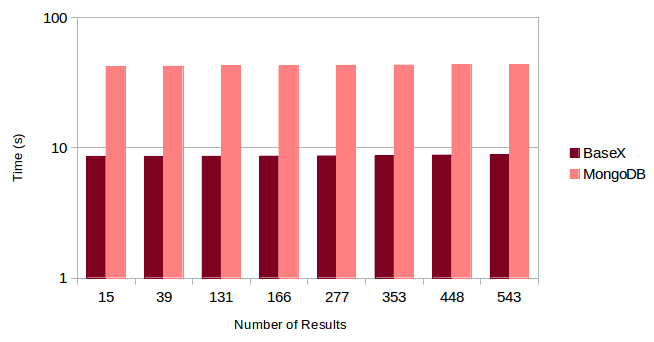
\includegraphics[width=0.8\textwidth,height=0.25\textheight]{BXvsMongo-NoIndex-Intersects-Sec-log}
%\caption{Query timing of \textit{intersect} operation without geospatial index}
%\label{figBXvsMongoNoIndexIntersects}
%\end{figure}


Until now, the sample queries are applied to the databases without using any index. 
In the following section, we measure the running time again by applying the geospatial index.
In this way, we also cover \textit{near} and \textit{nearSphere} queries in MongoDB that definately need the geospatial index.  
%using the \textit{distance} function to find the near geometries in BaseX in which the current index structure is not applicable.


%%%%%%%%%%%%%%%%%%%%%%%%%%%%%%%%%%%%%%
%%%% Section: Indexing in the Databases
%%%%%%%%%%%%%%%%%%%%%%%%%%%%%%%%%%%%%%
\subsection{Indexing in the Databases}
\label{index}
The assessment process is continued by applying the geospatial index. In MongoDB there are two choices for using geospatial index, \textit{2d} for data expressed in legacy coordinate pairs and \textit{2dsphere} for both GeoJSON data objects and legacy coordinate pairs. We use \textit{2dsphere} which fits to the choice of sherical maps via the following shell command,
\vspace{10px}
\begin{fakeJSON}
db.Collection.ensureIndex({geometry:"2dsphere"}) 
\end{fakeJSON}
\vspace{10px}
The same step is also taken in BaseX. Running again the same queries using a geospatial index, supposedly gives declined query times (see Figure~\ref{figBXvsMongoIndexIntersects}). As explained in Section~\ref{s.basex}, index is applied through the \textit{filter} function in BaseX while MongoDB follows another approach. MongoDB applies the index in casual query formats after executing the above-mentioned command and there is no need to change the queries in general. 

\begin{figure}
\centering
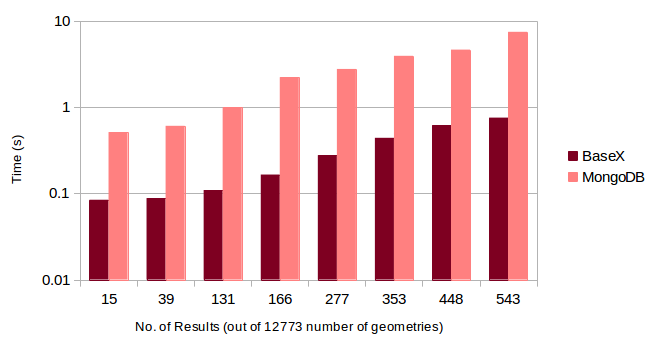
\includegraphics[width=0.8\textwidth]{BXvsMongo-Intersects-Index-Sec-log}
\caption{Query timing of \textit{intersect} operation with geospatial index}
\label{figBXvsMongoIndexIntersects}
\end{figure}

%Besides, the search for the geometries within an input area is done in the same way and the timings are shown in Figure~\ref{figBXvsMongoIndexWithin}. It can be seen that the queries with smaller number ofreturned geometries have better performane in MongoDB. Although it seems a positive point to return the big numbers of result in as shorter time as possible, considering smaller returned numbers of results is of greate importance for us, since these queries are more common in real-world usecases.

% TODO
%\begin{figure}
%\centering
%\includegraphics[width=0.7\textwidth]{BXvsMongo-Within-Index}
%\caption{Query timing of \textit{intersect} operation with geospatial index}
%\label{figBXvsMongoIndexIntersects}
%\end{figure}

The next widely used type of query is finding the near places or geometries up to a distance from a specific point. It could be also expressed as finding the geometries inside a circle with the distance value as the radius lenght. This feature is provided in MongoDB via \textit{\$near} and \textit{\$nearSphere} operators which simply get the reference point and the disance and hereafter returns the whole geometries in the specified distance from the point. Both near operators need a geospatial index, either \textit{2d} or \textit{2dsphere}. A specific distance in meter is defined as a condition to filter those geometries within this area. Below, we provide a sample query of the \textit{\$nearSphere} oprator.  
\vspace{10px}
\begin{fakeJSON}
db.collection.find({{geometry:
                       {$nearSphere:
                         {$geometry:
                           {type:"Point", coordinates:[4.5,51.95]}, 
                             $maxDistance : 100
                    }}}})
\end{fakeJSON}
\vspace{10px}
%TODO:reference for projected coordinate sys.
BaseX Geo Module currently provides this feature via \textit{distance} or combination of \textit{buffer} and \textit{within} functions. In Both cases, if the coordinate system in which the data is provided is a projected coordinate system, the distance can be specified in meter or any other metric unit. In a projected coordinate system, all the areas, lengths, and angels are defined on a flat two-dimensional space. In such a system, the user is provided with this \textit{near} feature in BaseX by using the above-mentioned functions as belows,
\vspace{10px}
\begin{fakeJSON}
import module namespace geo = "http://expath.org/ns/Geo";
declare namespace gml="http://www.opengis.net/gml";
let $a:= <gml:Point>
              <gml:coordinates>
               4.5,51.95 
               </gml:coordinates>
            </gml:Point>
for $b in //gml:Polygon 
return if (geo:distance( $a, $b) le 500) then $b else ()
\end{fakeJSON}
\vspace{10px}


For the data provided in a geographic coordinate system, calculations do not work with the metric values. A geographic coordinate system, such as WGS84, defines the areas and locations in a three-dimensional spherical space. Since there is not a specific unit for the current Geo Module functions, the \textit{distance} function interprets the input distance in the coordinate system of data. For example, the Netherlands sample dataset is in a metric coordinate system. Hence, the distance value in queries can be specified in meters. %TODO:better description

\begin{figure}
\centering
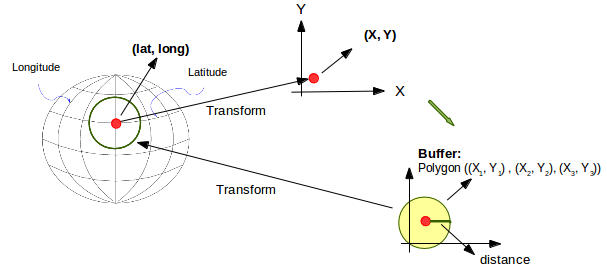
\includegraphics[width=\textwidth]{Transform}
\caption{Having the \textit{near} feature for WGS84 data using transformation in BaseX}
\label{figTransform}
\end{figure}

The aforementioned \textit{near} feature as a common use case is available in BaseX only for metric coordinate systems. To provide this feature also for geographic systems via the current geo functions, we need to convert the geographic coordinates to metric ones. In this way, we convert the specified input geometry in WGS84 to a metric system. Then, we compute the buffer of converted geometry up to the input distance in the same metric system and convert the buffer back to the original geographic coordinate system. A buffer of geometry is an identified region within a specific distance of the geometry. At the end, we find the all geometries within the buffer in geographic coorsinate system. This approach benefits from the geospatial index structure via the \textit{within} function while the approach with the \textit{distance} function do not utilize the geospaial index. This process is illustrated in Figure~\ref{figTransform}. 
This procedure is expressed as below, using the \textit{buffer} and \textit{within} functions and should return the same result as the previous query, 

\vspace{10px}
\begin{fakeJSON} 
within(geometry,
       transform(buffer(
                   transform(myPoint_in_wgs84, other_metric_cs)
                   , 500)
                 , wgs84
                )
      )
\end{fakeJSON}
\vspace{10px}
Having the same use cases, we have tested this feature in both databases, with the timing result shown in Figure~\ref{figBXvsMongoNear}. BaseX uses the distance function while \textit{\$nearSphere} operator finds the geometries in MongoDB. Obviously, MongoDB has a better performance, specifically with smaller number of results. The qurey times and the number of results are directly proportional in MongoDB, since the geospatial index is used and both chaneges accompany each other. BaseX do not use the geospatial index and consequently returns every result more or less in the same time.

%TODO: figure for converion method in BX
%TODO:change the chart for new queries of distance in BaseX


\begin{figure}
\centering
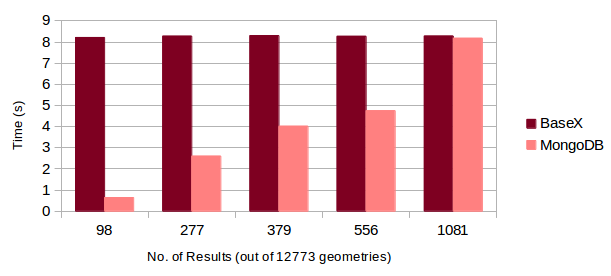
\includegraphics[width=0.8\textwidth]{BXvsMongoNear-newColor.png}
\caption{Query timing of the \textit{near} feature}
\label{figBXvsMongoNear}
\end{figure}


As mentioned in Section~\ref{indexBX}, BaseX records the index structure in a file and reads it back into main memory when the geospatial index is required. A Point which we should contemplate is to include the time for index opening in query times, since in memory management the index file might be removed from the memory and read back again. This time is not counted in the presented charts.
%TODO: better explanation


\subsection{Database Update}
\label{update}
%TODO:Complete!not good :|
Updating a database as a significant interaction supplied by the database system generally comprises three different operations: insert, delete, and modify. In addition to the whole issues related to the database update on disk and memory management, reconstructing the indexes is of great importance. That is, since the index is constructed based on the old database state, the updated database needs a new index. %ya masal

Currently in BaseX, updating is not applied to the geospatial index after the database update operations. It means that the STR-tree do not get updated automatically and the geospatial index has to be rebuilt manually. It causes redundant constructions and consequently worse performance. Here, we see how it could effect the updating performance in comparison with MongoDB which manages to rebuild the index in the updating process.

Considering the manual update of the geospatial index in BaseX, reindexing time must be examined to evaluate the updating process. This implies that the index creation time plus reopeneing the index file into the main memory should be included in the evaluation. 
Figure~\ref{figBXvsMongoUpdate} illustrates that the performance of all update operations in MongoDB are apparantly better. As mentioned before, reindexing in BaseX causes a huge growth in time, which individually takes the greatest amount of total time (see Figure~\ref{figBXUpdate}). We skip the result of deletion and insertion since they follow the similar pattern as update.

The unsatisfactory performance of the updating and also the \textit{near} feature in BaseX lead us to a new approach to use the MongoDB geospatial index from BaseX. The strategy is explained in the next section.

%TODO this is some part that we can speak about it in Conclusion
%Since the current index implementation do not involves updating based on the STR-tree definition, hence a new index should be designed and implemented.................
 


\begin{figure}
\centering
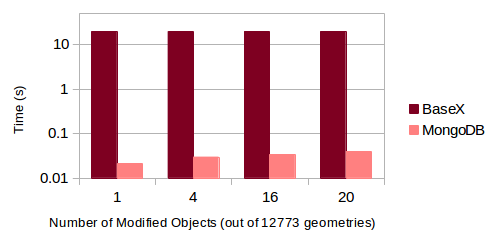
\includegraphics[width=0.7\textwidth]{BXvsMongo-Update-sec.png}
\caption{Performance of the \textit{update} operation in BaseX and MongoDB}
\label{figBXvsMongoUpdate}
\end{figure}


\begin{figure}
\centering
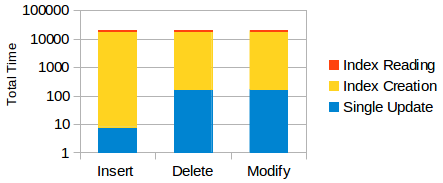
\includegraphics[width=0.7\textwidth]{BXUpdate.png}
\caption{Time consumtion percentage of the update operations in BaseX}
\label{figBXUpdate}
\end{figure}

\subsection{Querying by MongoDB via BaseX}
\label{MongoviaBX}
Up to this point we have investigated both BaseX and MongoDB to gain some improvement ideas for BaseX. We go further in this way by querying the data with MongoDB through BaseX. A conceivable goal for this approach could be supplying the missing features or make the features with better performance in MongoDB accessible from BaseX. In this approach, BaseX could be used as a connector to MongoDB, then the provided queries in MongoDB syntax are executed by MongoDB and the results are shown through BaseX. For the missing feature, this would add a functionality to BaseX. But, for the common queries we should evaluate the new query times to see how the performance changes. 
The test implementation is done by defining a connection string and the intended query in a function. However, these tasks could be specified through the XQuery by user and we just have done it as a test. 
In regards to the unsatisfactory query times in the \textit{near} feature, we have tried the \textit{\$nearSphere} operator. The performance modification of this feature is demonstrated in Figure~\ref{figMongoviaBX-near}.
 
\begin{figure}
\centering
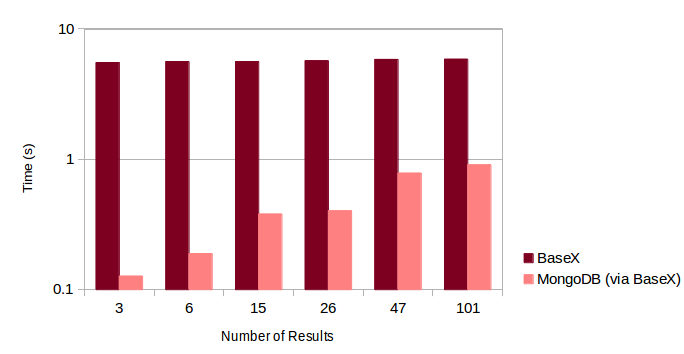
\includegraphics[width=0.9\textwidth]{MongoviaBX-near-sec-log.png}
\caption{Performance comparision of the \textit{near} feature in BaseX vs. MongoDB through BaseX}
\label{figMongoviaBX-near}
\end{figure}

Figure~\ref{figMongoviaBX-near} implies that the performance of \textit{near} query executed by MongoDB is preferable. The constant performance trend in BaseX is due to the absence of geospatial index. Hence, the user can benefit from this functionality in MongoDB through BaseX. 


\begin{figure}
\centering
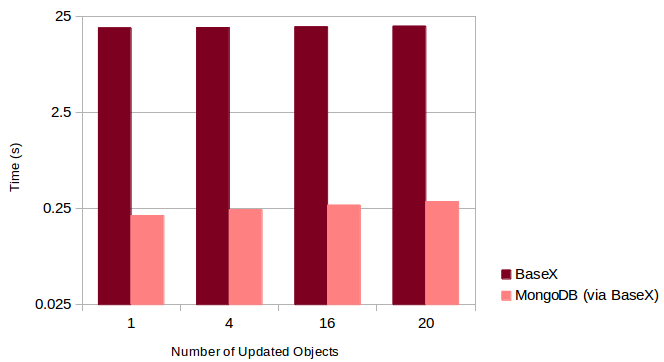
\includegraphics[width=0.8\textwidth]{MongoviaBX-Update-sec-log.png}
\caption{Performance comparision of the update operation in BaseX vs. MongoDB through BaseX}
\label{figMongoviaBX-update}
\end{figure}

This process is done for the update operaions such that the update query modifies the database in MongoDB. Correspondingly, it should be decided to continue the querying either in MongoDB or in BaseX after repeating the update queries and rebuilding the index structure. Figure~\ref{figMongoviaBX-update} indicates the better timing result of updating by MongoDB through BaseX. 

\subsection{Discussion}
\label{s.disc}
Throughout this section we investigated two strategies to efficiently process the geospatial data in BaseX. Based on these investigations, here we will discuss the  previously-mentioned approaches of the geospatial processing in BaseX and cover the pros and cons of the available approaches, particularly the most recent one in Section~\ref{MongoviaBX}. 

To start with, we suppose that a user has a geospatial dataset in GML and they would like to work in this format in BaseX, since their general requirements are met by BaseX. Based on our examinations, there are some queries in which BaseX is not able to cover them or can not provide some features in a proper timing. It means, those cases either are not covered, like updating the index structure or are covered with an apparently poor performance in comparision with the other similar query times, such as the \textit{near} feature. Therefore, geospatial queries such as \textit{intersects} or \textit{within}, can be applied efficiently while some other like \textit{near} and update, can not. Furthermore, regarding to our assumption, some funtionalities of BaseX convinces the user to work with GML. We call them \textit{GML-related} features. We consider these co-called \textit{GML-related} features in our discussion, as they might influnce the geospatial processing approch that wil be preferred.

%Although BaseX can handle the non-geospatial queries as well as some geospatial queries like intersects %and within almost efficiently using Index, the near query and the database update decreases the efficiency dramatically. Therefore, besides the geospatial queries there might be some non-geospatial queries as well, e.g. finding the point elements or the number of polygons in a dataset. It means that the geospatial queries are not necessarily the only focuse of the queries and the user can mix both types in a piece of code. Hence, these so-called non-geospatial queries should be considered in the set of user requiremets, however analysing them are not our focuse. This point is important when the user wants to choose between BaseX and MongoDB for geospatial queries while the non-geospaial queries will be done by BaseX. In this case the user can benefi from both databases while the most requirements are fulfilled by BaseX. 

%To summarize the results of our investigations, the near query and the geospatial index updating in BaseX are far from the ......???, though geospatial query times which are the focuse of the index structure, like intersects, seem that could be satisfying in some cases/some how.???  

Table~\ref{t.comparisonBaseXMongo} summarizes the statement above. \textit{MongoDB through BaseX} in this table means that BaseX connects to MongoDB to benefit by the features which are not available or available with poor performance in BaseX, as discussed in Section~\ref{MongoviaBX}. \textit{GML-related} features points the aforementioned features which are supposed here to be satisfying enough for the user, indicatd with the notation $"\times"$. This assumption is made in order to concentrate on the evaluation of those cases in which the user choose to use BaseX and we try to cover the missing geospatial features.
%Otherwise, the user might choose to work with another system, like MongoDB.
% is better in efficiency.
With $"\times\times"$, we mean that option is very efficient.
\vspace{10px}
\begin{table}
\centering
\begin{tabular}{|l | c | c|}\hline
\textbf{Tasks} & \textbf{BaseX} & \textbf{MongoDB through BaseX}\\\hline
 \textit{GML-related} Queries & $\times$ &\\\hline
 Geospatial Queries,  & $\times$ &\\
like \textit{intersects/within} & & \\\hline
 The \textit{near} Query & &$\times\times$ \\\hline
 DB Update Queries & &$\times\times$ 
%like update/insert/delete &&
\\\hline
\end{tabular}
\caption{The comparison of two strategies; using BaseX or connect to MongoDB via BaseX}
\label{t.comparisonBaseXMongo}
\end{table}
\vspace{10px}

As is expressed in Table~\ref{t.comparisonBaseXMongo}, the geospatial queries like \textit{intersects} and \textit{within} are working with an acceptable performance in BaseX. On the other hand, for the \textit{near} and update queries connecting to MongoDB seems to be the appropriate approach. Hence, a fast conclusion would be to have the advantage of using MongoDB through BaseX. However, the synchronization of the database instace in BaseX and the database instance in MongoDB should be precisely examined. If the user intends to modify the database which also means the modification of index without any further querying regarding the changes, the faster strategy is to update the MongoDB instace, while the database instance in BaseX remains untouched. But, in case that the user wants to do further querying based on the changes, this approach is not optimized.  

One way to discard the above-mentioned problem could be limiting the user to do all geospatial queries regarding the index in MongoDB and use BaseX just as a connector. 
However, as we see in Table~\ref{t.comparisonBaseXMongo} doing some queries in BaseX are more efficient and connecting to MongoDB might be a disadvantage, since this adds at least the connection time to the query time. Moreover, the complete dependency of BaseX on MongoDB for all geospatial queries would be too much and disadvantageous while each system is designed for different requirements and follow various goals. 
%a big limitation for this software regarding the geospatial processing. 
Thus, it will be more appropriate to provide the user with both possiblities.

Table~\ref{t.possibilities} summarizes the sample scenarios that could happen based on the existing features to process the geospatial data. In addition, this table shows the relevant/appropriate actions the user can apply as an efficient strategy toward her/his goal.


\begin{table}
\centering
\scalebox{1}{
\begin{tabular}{|l | l | }\hline
\textbf{Scenarios} & \textbf{What to do?}\\\hline
 Needs a \textit{instersects/within} query  & Using BaseX only\\
and no update and no \textit{near} query  & \\\hline
 Needs a \textit{near} query and no update & Using BaseX and MongoDB together\\\hline
 Needs modifications in the database & Using MongoDB only\\\hline
\end{tabular} }
\caption{Possible scenarios and appropriate actions suggested to take}
\label{t.possibilities}
\end{table}

The first scenario in Table~\ref{t.possibilities} is the use cases in which the BaseX \textit{Geo Module} functions and index structure fulfills all the requirements and there is no need for further queries, while the database remains unchaged. In such case, every thing could be done by BaseX. In the second scenario of this table the user needs the \textit{near} feature as a missing one, based on the untouched state of the database. For this case the user could connect to MongoDB in order to gain the result easier and faster. It should be mentioned that the issues related to the coordinate systems must be managed before applying the \textit{near} query. The last scenario mentioned in the table is the cases in shich the database will be updated and the next queries are based on the new state of the database. In this case which BaseX does not provide a proper way, accessing MongoDB update facilities and applying the subsequent queries in MongoDB hereafter is the advantageous approach. 

\subsection{Conclusion}
\label{conc}
In this section, we mainly concentrated on the geospatial features of MongoDB in order to find ways to improve the BaseX Geo Module efficiency. We started with the investigation of geospatial features to see the different viewpoints in MongoDB. Based on the common features in both databases, the perofrmances was represented and explained both with and without the index, to see the influence of geospatial index on them.
Among the queries, finding the geometries within a specific distance, called the \textit{near} feature, is of a great importance, as it is widely used. MongoDB provides this feature in both WGS84 for the data on Earth as well as legacy cordinate pairs, while BaseX supports only for the projected coordinate systems, since geospatial functions in BaseX do the calculation on the flat space. To add the support of data in WGS84 in BaseX, new functions should be implemented. Testing this feature in both databases shows better performance in MongoDB. 

%through \textit{\$near} and \textit{\$nearSphere} operators in MongoDB, while BaseX. 
Besides, updating in both databases is discussed. Update in MongoDB implicitly updates the index structure, while the geospatial index in BaseX must be reconstructed. Therefore, query time severly increases considering the time consumed by index updating. 


Since the performance of two major functionalities, i.e., the \textit{near} feature and updating, are not satisfying in BaseX and MongoDB provides them in a faster way, we connect to MongoDB and run these queries through BaseX. The results of the \textit{near} feature by this approach seem convincing enough to have this alternative way of querying in BaseX. In addition, updating the database by MongoDB via BaseX is faster than updating in BaseX. However, using this approach is controversial. The discussion is in regards to the subsequent queries after the database modification. Indeed, the changes happen in MongoDB and the database in BaseX remains untouched. Therefore, further querying based on the new changes is possible merely in MongoDB. In case that the next geospatial queries need to be done in BaseX, this way will not worth trying, because the whole update and index reconstruction process must be repeated in BaseX. The approach sets the limitation for the use cases in which the database will be updated, to do the geospatial querying completely in MongoDB.


\newpage
\section{Future Work}
\label{s.future}
We added to BaseX the new functionality of processing geospatial data.
However, there is still room for future improvements. 
In particular, the storage and indexings are in the center of attention.
Right now, the indexing tree is stored in the main memory 
which results in poor I/O efficiency.% reading time.
One of the first ideas is to bring some parts of the tree, 
which are addressed more, into RAM.
Regarding the indexing, an interesting future work is to practically compare 
the current STR-tree implementation with other indexing trees in the existence of
different kinds of geospatial data. For example, an interesting research would be
the comparison between STR-tree and Quadtree having dynamic datasets.
Moreover, the support of higher versions of GML and other geospatial data 
formats alike, could be a topic to work on.

In this thesis, we have considered MongoDB as an alternative for querying and indexing.
A feasible improvement would be the implementation of a flexible interface
for this database. As we discussed in Section~\ref{conc}, 
there would be an inconsistency between 
the geospatial data and indexing in BaseX and
the simultaneously indexed data in MongoDB. A future improvement is to 
implement a module to give the user the whole control over these two possibilities.
Besides, we can follow this idea by connection to the other well-known databases.

\newpage
\bibliographystyle{plain}
\bibliography{refs}
\newpage
\listoffigures
\newpage
\listoftables
\newpage
\lstlistoflistings

\end{document}	
